\documentclass[a4paper, oneside]{memoir}

\usepackage{imakeidx} % for clickable page numbers in index
\usepackage[colorlinks,citecolor=blue,linkcolor=blue,urlcolor=blue,]{hyperref} % for \href
\usepackage{dirtytalk} % for \say quotation
\usepackage{marginnote} % for margin notes
\usepackage{minipage-marginpar} % for the minipagewithmarginpars environment that allows marginpar commands in a minipage
\usepackage{amsfonts} % \mathbb
\usepackage[table]{xcolor} % coloring cells in tabular environments
\usepackage{minted} % for source code inclusion
\usepackage{attachfile2} % for attaching files to the PDF
\usepackage{pdfcomment} % for \pdftooltip command
\usepackage{layout} % for the \layout{} command used for debugging tikz
\usepackage{amsmath} % for aligned environment

% for subfigures
\usepackage{caption}
\usepackage{subcaption}

\usepackage{vissyntax}

%% attachfile2 symbol configuration
%\renewcommand{\atfi@acroPaperclip@data}{download}

% tikz
\usepackage{tikz}
\usetikzlibrary{patterns}
\usetikzlibrary{matrix}
\usetikzlibrary{decorations}
\usetikzlibrary{decorations.pathreplacing}

% configure index: https://en.wikibooks.org/wiki/LaTeX/Indexing
\usepackage{imakeidx}
\indexsetup{othercode=\small}
\makeindex[program=makeindex,columns=2,intoc=true,options={-s index_style.ist}]

\usepackage{fontspec}
\newfontface\lserif{Liberation Serif}

% biblatex setup
\usepackage[
  backend=biber,
]{biblatex}
\addbibresource{references.bib}

% tikz config
\usetikzlibrary{shapes,fit,calc}

% colors
\definecolor{lightblue}{HTML}{DEF2FB}
\definecolor{darkblue}{HTML}{BCE5FB}
\definecolor{lightbluetext}{HTML}{E6F7FF}
\definecolor{darkbluetext}{HTML}{D3EFFE}
\definecolor{bluetext}{HTML}{2E73A3}
\definecolor{grey}{HTML}{AFAFAF}

% styling
\setsecnumdepth{subsubsection} % how deep to number sections
\setlength{\parskip}{2mm} % vertical space between paragraphs
\setlength{\parindent}{0mm} % horizontal indent for first line of paragraph

\newcommand{\varname}[1]{\texttt{\textcolor{teal}{#1}}}
\newcommand{\typename}[1]{\texttt{\textcolor{purple}{#1}}}
\newcommand{\methodname}[1]{\texttt{\textcolor{blue}{#1}}}
\newcommand{\funcname}[1]{\methodname{#1}}
\newcommand{\packagename}[1]{\texttt{#1}}
\newcommand{\filename}[1]{\texttt{#1}}
\newcommand{\keywordname}[1]{\texttt{#1}}
\newcommand{\valuename}[1]{\texttt{#1}}
\newcommand{\commandname}[1]{\texttt{#1}}
\newcommand{\conceptname}[1]{\syntaxconceptcolor{#1}}

\newcommand{\langsection}[1]{\section{#1}}
\newcommand{\textdesc}[1]{\textit{\textbf{#1}}}
\newcommand{\descitem}[1]{\item \textdesc{#1}}
\newcommand{\quoted}[1]{\textsl{\say{#1}}}
\newcommand{\term}[1]{\textsl{#1}}

\newcommand{\csharp}{C{\lserif\#}}


\newcommand{\exercises}[2]{
  \input{exercises/#1.tex}
}

\newcommand{\includeCFile}[2][]{
  \begin{samepage}
    \marginpar{[\textattachfile{../src/c/#2}{\textcolor{blue}{extract file}}]}
    \inputminted[#1]{c}{../src/c/#2}
  \end{samepage}
}
\newcommand{\includeCsharpFile}[2][]{
  \begin{samepage}
    \marginpar{[\textattachfile{../src/csharp/#2}{\textcolor{blue}{extract file}}]}
    \inputminted[#1]{csharp}{../src/csharp/#2}
  \end{samepage}
}
\newcommand{\includeElixirFile}[2][]{
  \begin{samepage}
    \marginpar{[\textattachfile{../src/elixir/#2}{\textcolor{blue}{extract file}}]}
    \inputminted[#1]{elixir}{../src/elixir/#2}
  \end{samepage}
}
\newcommand{\includePythonFile}[2][]{
  \begin{samepage}
    \marginpar{[\textattachfile{../src/python/#2}{\textcolor{blue}{extract file}}]}
    \inputminted[#1]{python}{../src/python/#2}
  \end{samepage}
}

\newenvironment{inspiration}[2][0.9]
{
  \begin{center}
  \newcommand{\saveme}{#2}
  \begin{minipagewithmarginpars}{#1\textwidth}
}
{
  
  \raggedleft{--- \textsl{\saveme}}
  \end{minipagewithmarginpars}
  \end{center}
}

\newenvironment{syntaxsegment}[1][0.9]
{
  \begin{center}
    \begin{tabular}{|p{#1\textwidth}|}
      \hline
      \cellcolor[gray]{0.9}
      \textbf{Syntax} \\
      \hline
      \cellcolor[gray]{0.95}
}{
      \\
      \hline
    \end{tabular}
  \end{center}
}

\input{hlsections.tex}

% https://en.wikibooks.org/wiki/LaTeX/Indexing
%\newcommand{\idxx}[2]{\index{#1}\marginpar{\raggedright \tiny #2}}
\newcommand{\idx}[2]{\index{#2}\textcolor{purple}{#1}}
\newcommand{\idxx}[1]{\idx{#1}{#1}}
\newcommand{\defi}[2]{\index{#2|textbf}\textcolor{purple}{\underline{#1}}}
\newcommand{\defix}[1]{\defi{#1}{#1}}

% https://tex.stackexchange.com/questions/210435/adding-space-in-toc-between-the-part-number-and-part-title
\renewcommand\partnumberlinebox[2]{#2\hspace{1em}}

\newcommand{\context}[0]{this should be renewed to something useful}

\title{Introduction to Programming \ldots\ in \csharp}
\author{Aslak Johansen \href{mailto:asjo@mmmi.sdu.dk}{asjo@mmmi.sdu.dk}}

\begin{document}

% front matter
\maketitle
\setcounter{tocdepth}{2}
\tableofcontents
\newpage
\listoffigures
\newpage
\listofsyntaxfloat

% cross-index entries
\scalebox{0}{
  \textcolor{white}{\index{BNF|see {Backus-Naur Form}}}
  \textcolor{white}{\index{Digraph|see {Directed graph}}}
  \textcolor{white}{\index{Directed acyclic graph|see {DAG}}}
  \textcolor{white}{\index{Folder|see {Directory}}}
  \textcolor{white}{\index{N@$\mathbb{N}$|see {Numbers, natural}}}
  \textcolor{white}{\index{P@$\mathbb{P}$|see {Numbers, irrational}}}
  \textcolor{white}{\index{Q@$\mathbb{Q}$|see {Numbers, rational}}}
  \textcolor{white}{\index{R@$\mathbb{R}$|see {Numbers, real}}}
  \textcolor{white}{\index{Z@$\mathbb{Z}$|see {Numbers, integer}}}
  \textcolor{white}{\index{IR|see {Infra-red}}}
  \textcolor{white}{\index{UV|see {Ultra-violet}}}
  \textcolor{white}{\index{Raw text file|see {Text file}}}
}

\chapter*{Preface}
\addcontentsline{toc}{chapter}{Preface}

% my background: classical (experimental) computer science, programming language tolerant, teaching object oriented programming (java and csharp) on a danish SE education, what is a danish SE education.
My background is from fairly classical (experimental) computer science, and has always been programming language tolerent. Today, I am teaching an introductionary programming course on a Danish software engineering education. That course has a focus on object-orientation. Previously, the it targeted Java, but we recently made the shift to \csharp.

% why c#?
\csharp\ (and Java for that matter) are languages that mix the fundamentals with a great amount of complexity. From what I see, students have a tendency to loose track of those fundamentals. So, why teach such langauges on the first course on programming? Well, only about half of a Danish software engineering education is computer science. The rest is project management, customer relations, requirement analysis and similar fields that are peripheral to programming. That means that some shortcuts have to be taken. And this is one.

% motivation: lack of introduction-level C# books that doesn't try to bypass the learning experience
Many \csharp\ books already exist, and quite a few of them claim to be aimed a novices. But as far as I can tell, they all bypass learning experiences that I feel are essential to informing the understanding of the student. This book is intended to fill that gap.

\chapter{Introduction}
\label{sec:intro}

Hello

\section{Intended Audience}

\section{Tenets}

\begin{enumerate}
  \item The role of a course introducing programming is to create a technical foundation, not to please the industry. Ideally, students of such a course can -- in time -- bring positive change to the industry.
  \item Practice should be rooted in theory.
  \item The why is just as important as the how.
  \item Concepts are more important than concrete implementations.
  \item Concrete implementation choices can often be highlighted by contrasting to other implementations.
  \item Students should be able to look to educational material for good examples of how to write.
\end{enumerate}

\section{\idx{Reading Guide}{Reading guide}}

\subsection{Mindset}

\begin{inspiration}{\idx{Ralph Waldo Emerson}{Emerson, Ralph Waldo}\cite{selfrel}}
  \quoted{Its not the Destination, It's the journey.}
\end{inspiration}

% general: how we learn
People rarely decide to undertake the hardships of learning something because they want to go through the process of learning. They want have been through the process and know. It's the destination that pulls them in. As intelligent beings we subconsciously seek shortcuts, yet we are not particularly good at keeping the long-term goalpost present in mind. In order to absorb and understand the knowledge we need to be present along the way, observe the details and experience how they relate to each other. This applies to programming, perhaps more so than to most other fields.

% specific: this book positioned in your journey
This book is intended to help you in during the very first leg of your journey. As that is the first of many, focus will be on learning the basics rather than learning concrete tools and technologies that are used in the industry. At times these goals overlap, but more often than not they conflict. So, this book will not prepare you for the industry. That is a task you will have to deal with later on in your journey.

% specific: within this book

% your help needed
So, we need your help in achieving this. You do so by keeping a focus on the following across your studies:
\begin{enumerate}
  \descitem{Curiosity} 
  \descitem{Pride} 
  \descitem{Thoroughness} 
  \descitem{Effort} 
  \descitem{Communication} 
\end{enumerate}

\subsection{Index}

Items are grouped so that in order to look up a \say{directed edge}, one first looks up \say{edge}, and then \say{directed} among the related entries. Page numbers with definitions are marked with bold.

\section{Acknowledgments}

\chapter{Background}

Before we get started on installing the prereqs for this course, we need to cover some basic theory. This is not only relevant for installing the prereqs, but will pop up frequently throughout this course, and after it.

\section{Graphs}
\label{sec:bg:graph}

A \idx{graph}{Graph} is the combination of a set of nodes and a set of edges between these nodes. You could see the \idx{nodes}{Node} as \textsl{things} and the \idx{edges}{Edge} as \textsl{relationships between things}. But lets take a look at the concrete example of figure \ref{fig:bs:graphs:graph}. Here, we have nine nodes -- $n_1$ through $n_9$ -- and eleven edges. The layout of where the individual nodes a placed doesn't mater. So, we could flip the positions of $n_4$ and $n_7$ whichout changing the graph itself. Although, the representation of the graph would obviously change.

\begin{figure}[tbp]
  \input{figs/graph.tex}
  \caption{Example of a graph.}
  \label{fig:bs:graphs:graph}
\end{figure}

Edges may be \idx{directional}{Edge!Directed} as in figure \ref{fig:bs:graphs:directed}. This means that there is an edge from $n_1$ to $n_2$ but not the other way around. We say that the \idx{source node}{Node!Source} of this edge is $n_1$ and the \idx{destination node}{Node!Destination} is $n_2$. Another way to look at it is that this edge belong to the set of \idx{outgoing edges}{Edge!Outgoing} of $n_1$ as well as the set of \idx{incoming edges}{Edge!Incoming} of $n_2$. Most graphs in computer science consists of directed edges. If all edges in a graph are directed, then we say that the graph is \idx{directed}{Graph!Directed} or simply that it is a \textsl{digraph}.

\begin{figure}[tbp]
  \begin{center}
  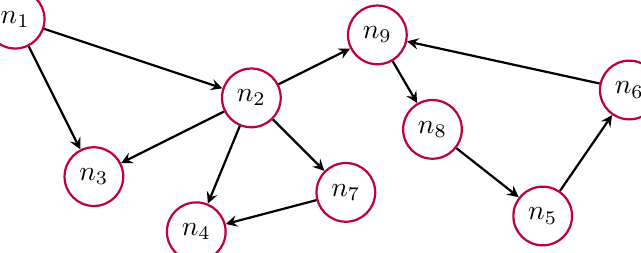
\begin{tikzpicture}[remember picture]
    \tikzstyle{edge}  = [thick,>=stealth,draw=black]
    \tikzstyle{dedge} = [thick,->,>=stealth,draw=black]
    \tikzstyle{node}=[
      overlay,
      circle,
      draw=purple,
      anchor=center,
      thick,
      minimum size=1,
    ]
    
    \node[node] (n1) at (-4,0) {$n_1$};
    \node[node] (n2) at (-1,-1) {$n_2$};
    \node[node] (n3) at (-3,-2) {$n_3$};
    \node[node] (n4) at (-1.7,-2.7) {$n_4$};
    \node[node] (n5) at (2.7,-2.5) {$n_5$};
    \node[node] (n6) at (3.8,-0.9) {$n_6$};
    \node[node] (n7) at (0.2,-2.2) {$n_7$};
    \node[node] (n8) at (1.3,-1.4) {$n_8$};
    \node[node] (n9) at (0.6,-0.2) {$n_9$};
    
    \draw[dedge] (n1)--(n2);
    \draw[dedge] (n2)--(n3);
    \draw[dedge] (n1)--(n3);
    \draw[dedge] (n2)--(n4);
    \draw[dedge] (n2)--(n9);
    \draw[dedge] (n9)--(n8);
    \draw[dedge] (n6)--(n9);
    \draw[dedge] (n5)--(n6);
    \draw[dedge] (n2)--(n7);
    \draw[dedge] (n7)--(n4);
    \draw[dedge] (n8)--(n5);
  \end{tikzpicture}
\end{center}

  \caption{Example of a directed graph.}
  \label{fig:bs:graphs:directed}
\end{figure}

Both nodes and edges can be associated with data. Edges, for instance, are often associated with \idx{weights}{Edge!Weighted}. Such a graph is called a \idx{weighted graph}{Graph!Weighted}. Figure \ref{fig:bs:graphs:weighted} illustrates such an example. Directed graphs can be used to model road networks. Each node is then a point of interest (e.g., a city or a crossing), and edges represents roads. The weight of an edge is the distance of that road. So, we might say that there is a distance of $1.1~\mathrm{km}$ from $n_9$ to $n_8$.

\begin{figure}[tbp]
  \input{figs/graph_weighted.tex}
  \caption{Example of a weighted graph.}
  \label{fig:bs:graphs:weighted}
\end{figure}

A routefinding application -- like Google Maps -- has access to a a weighted graph of some area. When you ask it for a route from $n_1$ to $n_6$ it will try to find a sequence of edges where the source node of one edge is the same as the destination node of the previous edge. Such a sequence is called a \idx{path}{Path}, and the resulting path is illustrated in figure \ref{fig:bs:graphs:path}.

\begin{figure}[tbp]
  \input{figs/graph_path.tex}
  \caption{Example of a path in a graph.}
  \label{fig:bs:graphs:path}
\end{figure}

Figure \ref{fig:bs:graphs:cycle} illustrates a special kind of path called a \idx{cycle}{Cycle|textbf}. This is a path where the destination node of the last edge is the same as the source node of the first edge. While they are often necessesary, their potential existence complicates the code of the programs that have to deal with them. For this reason we often see software designed to handle the class of graphs that have no cycles. These are called \textsl{Directed Acyclic Graphs}, or \idx{DAGs}{DAG} for short.

\begin{figure}[tbp]
  \begin{center}
  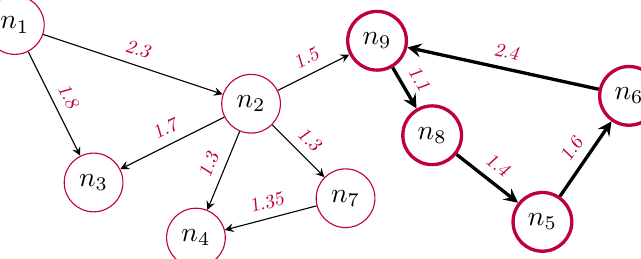
\begin{tikzpicture}[remember picture]
    \newcommand{\weight}[1]{node[midway,sloped,above] {\scalebox{0.7}{\textsl{\textcolor{purple}{#1}}}}}
    \tikzstyle{edge}  = [thick,>=stealth,draw=black]
    \tikzstyle{dedge} = [thick,->,>=stealth,draw=black]
    \tikzstyle{node}=[
      overlay,
      circle,
      draw=purple,
      anchor=center,
      thick,
      minimum size=1,
    ]
    
    \node[node,thin] (n1) at (-4,0) {$n_1$};
    \node[node,thin] (n2) at (-1,-1) {$n_2$};
    \node[node,thin] (n3) at (-3,-2) {$n_3$};
    \node[node,thin] (n4) at (-1.7,-2.7) {$n_4$};
    \node[node,very thick] (n5) at (2.7,-2.5) {$n_5$};
    \node[node,very thick] (n6) at (3.8,-0.9) {$n_6$};
    \node[node,thin] (n7) at (0.2,-2.2) {$n_7$};
    \node[node,very thick] (n8) at (1.3,-1.4) {$n_8$};
    \node[node,very thick] (n9) at (0.6,-0.2) {$n_9$};
    
    \draw[dedge,thin] (n1)--(n2) \weight{2.3};
    \draw[dedge,thin] (n2)--(n3) \weight{1.7};
    \draw[dedge,thin] (n1)--(n3) \weight{1.8};
    \draw[dedge,thin] (n2)--(n4) \weight{1.3};
    \draw[dedge,thin] (n2)--(n9) \weight{1.5};
    \draw[dedge,very thick] (n9)--(n8) \weight{1.1};
    \draw[dedge,very thick] (n6)--(n9) \weight{2.4};
    \draw[dedge,very thick] (n5)--(n6) \weight{1.6};
    \draw[dedge,thin] (n2)--(n7) \weight{1.3};
    \draw[dedge,thin] (n7)--(n4) \weight{1.35};
    \draw[dedge,very thick] (n8)--(n5) \weight{1.4};
  \end{tikzpicture}
\end{center}

  \caption{Example of a cycle in a graph.}
  \label{fig:bs:graphs:cycle}
\end{figure}

% reachability, connected graph

\subsection{Trees}

A connected graph with $n$ nodes has at least $n-1$ edges. If it has exactly $n-1$ edges then it belongs to the class of graphs called \idx{trees}{Tree}. Trees are traditionally drawn upside down, like in figure \ref{fig:bs:graphs:trees}. Just as with other graphs, we have some liberty in how to draw the nodes and edges. Here, we have left out the identities of the individual nodes.

\begin{figure}[tbp]
  \input{figs/graph_tree.tex}
  \caption{Example of a tree.}
  \label{fig:bs:graphs:trees}
\end{figure}

A special node of the tree is called the \idx{root node}{Node!Root}. It is drawn at the top of the illustration, and it has exactly one path the each of the other nodes of the graph. As illustrated in figure \ref{fig:bs:graphs:trees:nodetypes}, each of the nodes in a tree are often categorized as either \idx{leaf nodes}{Node!Leaf} (with no outgoing edges) or \idx{branch nodes}{Node!Branch} (typically with outgoing edges).

\begin{figure}[tbp]
  \begin{center}
  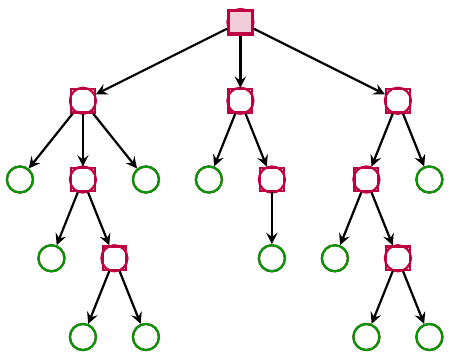
\begin{tikzpicture}[remember picture]
    \newcommand{\weight}[1]{node[midway,sloped,above] {\scalebox{0.7}{\textsl{\textcolor{purple}{#1}}}}}
    
    \tikzstyle{edge}  = [thick,>=stealth,draw=black]
    \tikzstyle{dedge} = [thick,->,>=stealth,draw=black]
    \tikzstyle{snode}=[
      overlay,
      circle,
      draw=purple,
      anchor=center,
      thick,
      minimum size=0.2,
    ]
    \tikzstyle{snoded}=[
      snode,
      rectangle,
      minimum width=0.3cm,
      minimum height=0.3cm,
    ]
    \tikzstyle{leaf}=[
      snode,
      draw=green!60!black,
    ]
    
    {
      \node[snode] (n1) at (0,0) {};
      
      \node[snode] (n11) at (-2.0,-1) {};
      \node[snode] (n12) at (0,-1) {};
      \node[snode] (n13) at (2.0,-1) {};
      
      \node[snode] (n111) at (-2.8,-2) {};
      \node[snode] (n112) at (-2.0,-2) {};
      \node[snode] (n113) at (-1.2,-2) {};
      \node[snode] (n121) at (-0.4,-2) {};
      \node[snode] (n122) at (0.4,-2) {};
      \node[snode] (n131) at (1.6,-2) {};
      \node[snode] (n132) at (2.4,-2) {};
      
      \node[snode] (n1121) at (-2.4,-3) {};
      \node[snode] (n1122) at (-1.6,-3) {};
      \node[snode] (n1221) at (0.4,-3) {};
      \node[snode] (n1311) at (1.2,-3) {};
      \node[snode] (n1312) at (2.0,-3) {};
      
      \node[snode] (n11221) at (-2.0,-4) {};
      \node[snode] (n11222) at (-1.2,-4) {};
      \node[snode] (n13121) at (1.6,-4) {};
      \node[snode] (n13122) at (2.4,-4) {};
    }
    
    {
      \node[snoded, very thick,fill=purple!20] (n1) at (0,0) {};
    }
    
    {
      \node[snoded] (n11) at (-2.0,-1) {};
      \node[snoded] (n12) at (0,-1) {};
      \node[snoded] (n13) at (2.0,-1) {};
      
      \node[leaf] (n111) at (-2.8,-2) {};
      \node[snoded] (n112) at (-2.0,-2) {};
      \node[leaf] (n113) at (-1.2,-2) {};
      \node[leaf] (n121) at (-0.4,-2) {};
      \node[snoded] (n122) at (0.4,-2) {};
      \node[snoded] (n131) at (1.6,-2) {};
      \node[leaf] (n132) at (2.4,-2) {};
      
      \node[leaf] (n1121) at (-2.4,-3) {};
      \node[snoded] (n1122) at (-1.6,-3) {};
      \node[leaf] (n1221) at (0.4,-3) {};
      \node[leaf] (n1311) at (1.2,-3) {};
      \node[snoded] (n1312) at (2.0,-3) {};
      
      \node[leaf] (n11221) at (-2.0,-4) {};
      \node[leaf] (n11222) at (-1.2,-4) {};
      \node[leaf] (n13121) at (1.6,-4) {};
      \node[leaf] (n13122) at (2.4,-4) {};
    }
    
    {
      \draw[dedge] (n1)--(n11);
      \draw[dedge] (n1)--(n12);
      \draw[dedge] (n1)--(n13);
      
      \draw[dedge] (n11)--(n111);
      \draw[dedge] (n11)--(n112);
      \draw[dedge] (n11)--(n113);
      \draw[dedge] (n12)--(n121);
      \draw[dedge] (n12)--(n122);
      \draw[dedge] (n13)--(n131);
      \draw[dedge] (n13)--(n132);
      
      \draw[dedge] (n112)--(n1121);
      \draw[dedge] (n112)--(n1122);
      \draw[dedge] (n122)--(n1221);
      \draw[dedge] (n131)--(n1311);
      \draw[dedge] (n131)--(n1312);
      
      \draw[dedge] (n1122)--(n11221);
      \draw[dedge] (n1122)--(n11222);
      \draw[dedge] (n1312)--(n13121);
      \draw[dedge] (n1312)--(n13122);
    }
  \end{tikzpicture}
\end{center}

  \caption{Node types of a tree.}
  \label{fig:bs:graphs:trees:nodetypes}
\end{figure}

Trees are typically used for searching or representing hierarchical data. This could be a taxonomy tree, or the \textsl{nesting} of elements in a graphical user interface.


\section{Filesystems}
\idx{Filesystem}

% what(for a computer)
Most computers organize persisted data in files. That the data are persisted\idx{Persistence} means that the data will survive a power cycle\idx{Power cycle} of the computer (i.e., that it is turned off and on again). All data available to the operating system (includin programs and configuration) is stored in files.

% what: tree
Filesystems are \textsl{mostly} tree structures, organizing files in directories. A directory\idx{Directory} is a special form of file that can group other files. In tree terminology, they are branch nodes whereas ordinary files are leaf nodes. The visual metaphore that graphical user interfaces use to refer to directories is the folder. But at the filesystem level -- which is what we care about as programmers -- it is a directory. Figure \ref{fig:bs:fs} shows what a typical filesystem could look like.

\begin{figure}[tbp]
  \input{figs/fs.tex}
  \caption{Example of a filesystem.}
  \label{fig:bs:fs}
\end{figure}

\subsection{Mounting}

Removable media, like a USB drive, are usually formatted to contain a filesystem. That is why we can place images and documents on it. In order to access that filesystem on your computer it must be mounted once attached. A mount\idx{Mounting} operation essentially makes a specific directory -- the mountpoint\idx{Mount point} -- a shorthand of the root of the mounted filesystem, thereby practically grafting the mounted filesystem to the root\idxx{Filesystem!Root}{Root filesystem} filesystem. The result of the mount operation is illustrated in figure \ref{fig:bs:fs:mounting}. On DOS\idx{DOS}-based systems (such as the Windows\idx{Windows} family of operating systems),
each known filesystem is assigned a letter, and a (hidden) root directory refers
to each of these.

\begin{figure}[tbp]
  \input{figs/fs_mounting.tex}
  \caption{Example of a mounting a guest filesystem.}
  \label{fig:bs:fs:mounting}
\end{figure}

\subsection{Links}

Modern filesystems support links though, and that is a feature that makes them break their adherence to the tree definition. A link is a special kind of file that refers to an other file (regular or directory). Figure \ref{fig:bs:fs:links} shows a scenario where a link refers to a regular file. That means that we have two paths from the root node to this regular file; one that goes through the link and one that doesn't. That means that the filesystem is no longer a tree structure. As illustrated in figure \ref{fig:bs:fs:cycles}, a link can also go backward. By pointing to a directory earlier in the path from the root node to the link node a cycle is created. This will complicate things if we need to scan the entire filesystem. Because of this, you often see commandline tools have options for following or not following links.

While modern versions of the Windows family of operating systems does have some support for links, it can be sketchy. Instead they support \textsl{shortcuts} through a special \filename{LNK} file format. The content of a file following this format is a path to a file that the link points to. While this solution is a bit more flexible, it has to be interpreted by each application instead of the filesystem and is thus harder to work with and less performant.

\begin{figure}[tbp]
  \input{figs/fs_links.tex}
  \caption{Example of a link in a filesystem.}
  \label{fig:bs:fs:links}
\end{figure}

\begin{figure}[tbp]
  \input{figs/fs_cycles.tex}
  \caption{Example of how a link can create a cycle in a filesystem.}
  \label{fig:bs:fs:cycles}
\end{figure}

\begin{figure}[tbp]
  \input{figs/fs_path_abs.tex}
  \caption{Example of an absolute path in a filesystem.}
  \label{fig:bs:fs:path:abs}
\end{figure}

\subsection{Paths}

\begin{figure}[tbp]
  \input{figs/fs_path_rel.tex}
  \caption{Example of an relative path in a filesystem.}
  \label{fig:bs:fs:path:rel}
\end{figure}


\section{Processes}

\subsection{Kernel}

\subsection{Desktop Environment}

\subsection{Shell}

\subsection{Working with Files}

\subsubsection{Copying Files}

\begin{figure}[tbp]
  \begin{center}
  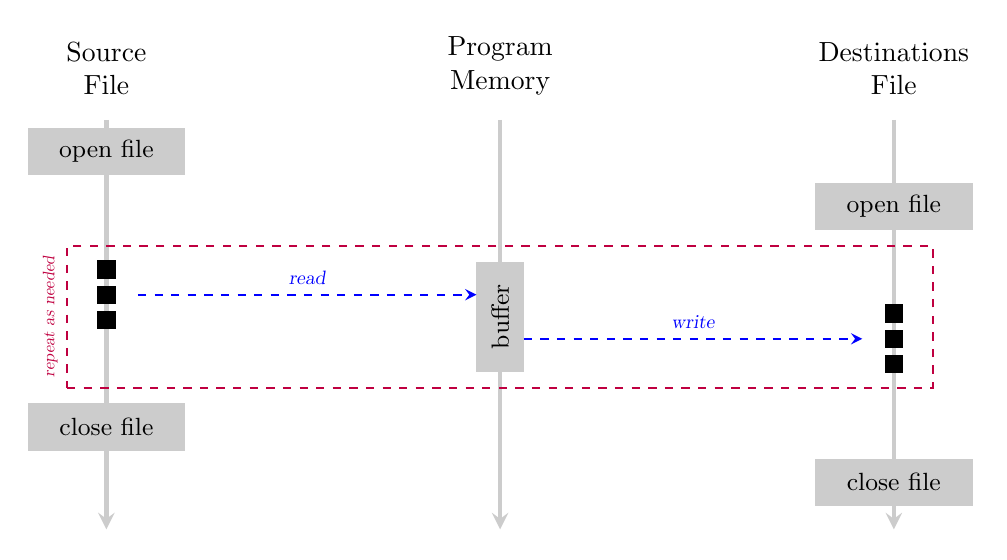
\begin{tikzpicture}[remember picture]
    \tikzstyle{title} = [
      anchor=south,
      align=center,
    ]
    \tikzstyle{arrow} = [
      thick,
      ->,
      >=stealth,
      draw=black,
    ]
    \tikzstyle{fileline}=[
      arrow,
      ultra thick,
      draw=black!20,
    ]
    \tikzstyle{fd} = [
      anchor=center,
      align=center,
      fill=black!20,
      minimum width=2cm,
      minimum height=0.6cm,
    ]
    \tikzstyle{data} = [
      anchor=center,
      fill=black,
      minimum width=1.5mm,
      minimum height=1.5mm,
    ]
    
    \newcommand{\shiftdistance}[0]{5cm}
    \newcommand{\figheight}[0]{5.2cm}
    
    \coordinate (memAnchor) at (0,-1cm);
    \coordinate (srcAnchor) at ([xshift=-\shiftdistance, yshift=0] memAnchor);
    \coordinate (dstAnchor) at ([xshift= \shiftdistance, yshift=0] memAnchor);
    
    % src line
    {
      \node[title] (srcTitle) at ([yshift=2mm] srcAnchor) {Source\\File};
      \draw[fileline] (srcAnchor) -- ([yshift=-\figheight] srcAnchor);
    }
    
    % dst line
    {
      \node[title] (dstTitle) at ([yshift=2mm] dstAnchor) {Destinations\\File};
      \draw[fileline] (dstAnchor) -- ([yshift=-\figheight] dstAnchor);
    }
    
    % mem line
    {
      \node[title] (memTitle) at ([yshift=2mm] memAnchor) {Program\\Memory};
      \draw[fileline] (memAnchor) -- ([yshift=-\figheight] memAnchor);
    }
    
    % open(src)
    {
      \node[fd] (srcOpen) at ([yshift=-4mm] srcAnchor) {\small{open file}};
    }
    
    % open(dst)
    {
      \node[fd] (dstOpen) at ([yshift=-11mm] dstAnchor) {\small{open file}};
    }
    
    % buffer
    {
      \node[fd, minimum width=0.6cm, minimum height=1.4cm] (buffer) at ([yshift=-25mm] memAnchor) {\rotatebox{90}{\small{buffer}}};
    }
    
    % read
    {
      \node[data] (srcDataI)   at ([yshift=-19mm] srcAnchor) {};
      \node[data] (srcDataII)  at ([yshift=-3.2mm] srcDataI) {};
      \node[data] (srcDataIII) at ([yshift=-3.2mm] srcDataII) {};
      
      \draw[arrow, dashed, draw=blue]
        ([xshift=4mm] srcDataII.center)--([xshift=\shiftdistance-0.3cm] srcDataII.center)
        node[midway,sloped,above]
        {\scalebox{0.7}{\textsl{\textcolor{blue}{read}}}};
    }
    
    % write
    {
      \node[data] (dstDataIII) at ([yshift=-31mm] dstAnchor) {};
      \node[data] (dstDataII)  at ([yshift=3.2mm] dstDataIII) {};
      \node[data] (dstDataI)   at ([yshift=3.2mm] dstDataII) {};
      
      \draw[arrow, dashed, draw=blue]
        ([xshift=-\shiftdistance+0.3cm] dstDataII.center)--([xshift=-4mm] dstDataII.center)
        node[midway,sloped,above]
        {\scalebox{0.7}{\textsl{\textcolor{blue}{write}}}};
    }
    
    % repetition
    {
      \node[rectangle, thick, dashed, draw=purple, anchor=center, minimum width=2*\shiftdistance+10mm, minimum height=1.8cm] (repetition) at ([yshift=-25mm] memAnchor) {};
      \node[] (repetitionLabel) at ([xshift=-2mm] repetition.west) {\rotatebox{90}{\scalebox{0.60}{\textsl{\textcolor{purple}{repeat as needed}}}}};
    }
    
    % close(src)
    {
      \node[fd] (srcOpen) at ([yshift=-39mm] srcAnchor) {\small{close file}};
    }
    
    % close(dst)
    {
      \node[fd] (dstOpen) at ([yshift=-46mm] dstAnchor) {\small{close file}};
    }
  \end{tikzpicture}
\end{center}

  \caption{How a file is copied.}
  \label{fig:bg:processes:copy}
\end{figure}

\subsubsection{Editing Files}

\section{File Formats}

% intro
Data is stored in files and they are organized in directories on in a filesystem. 

\begin{figure}[tbp]
  \section{File Formats}

% intro
Data is stored in files and they are organized in directories on in a filesystem. 

\begin{figure}[tbp]
  \input{figs/background_fileformats.tex}
  \caption{The relationship between programs, file formats and functions.}
  \label{fig:bg:fileformats}
\end{figure}

  \caption{The relationship between programs, file formats and functions.}
  \label{fig:bg:fileformats}
\end{figure}

\section{The Machine}
\label{sec:machine}

\subsection{History}

% Antikythera mechanism https://en.wikipedia.org/wiki/Antikythera_mechanism

% Jacquard machine https://en.wikipedia.org/wiki/Jacquard_machine

% Difference Engine https://en.wikipedia.org/wiki/Difference_engine

% Mutual Exclusion https://en.wikipedia.org/wiki/Mutual_exclusion

% C https://en.wikipedia.org/wiki/C_(programming_language)

% Taming of the Alpaca

\subsection{Overview}

% description of computer: model description as data flow (input, memory, processor, load instruction, registers, operator instructions, ALU, store instruction, memory, output)
Figure \ref{fig:machine:computer}

\begin{figure}[tbp]
  \begin{center}
  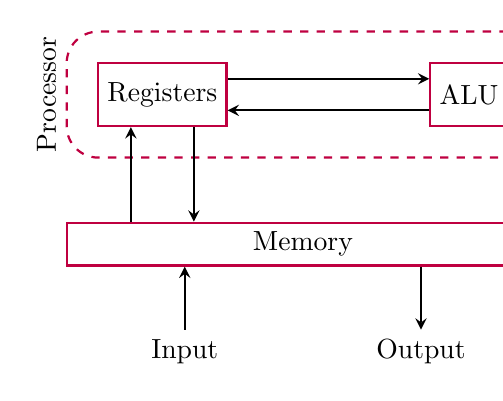
\begin{tikzpicture}[remember picture]
    \newcommand{\spacing}[0]{ 8mm }
    \tikzstyle{edge}  = [thick,>=stealth,draw=black]
    \tikzstyle{dedge} = [thick,->,>=stealth,draw=black]
    \tikzstyle{node}=[
      overlay,
      rectangle,
      draw=purple,
      anchor=center,
      thick,
    ]
    
    \node[node,minimum height=2*\spacing,minimum width=6cm,rounded corners=4mm,dashed] (processor) at (0,0) {};
    \node[anchor=east] (processor_label) at
      (processor.west)
      {\rotatebox{90}{Processor}};
    \node[node,anchor=north west,minimum height=\spacing] (registers) at
      ([xshift=0.5*\spacing,yshift=-0.5*\spacing]processor.north west)
      {Registers};
    \node[node,anchor=north east,minimum height=\spacing] (alu) at
      ([xshift=-0.5*\spacing,yshift=-0.5*\spacing]processor.north east)
      {ALU};
    \node[node,anchor=north,minimum width=6cm] (memory) at
      ([yshift=-\spacing]processor.south)
      {Memory};
    \node[anchor=north] (input) at
      ([xshift=-1.5cm,yshift=-\spacing]memory.south)
      {Input};
    \node[anchor=north] (output) at
      ([xshift=1.5cm,yshift=-\spacing]memory.south)
      {Output};
    
    % register <-> alu
    \draw[dedge] ([yshift= 2mm]registers.east)
               --([yshift= 2mm]alu.west);
    \draw[dedge] ([yshift=-2mm]alu.west)
               --([yshift=-2mm]registers.east);
    
    % register <-> memory
    \draw[dedge] ([xshift=-4mm,yshift=-1.5*\spacing]registers.south)
               --([xshift=-4mm]                     registers.south);
    \draw[dedge] ([xshift= 4mm]                     registers.south)
               --([xshift= 4mm,yshift=-1.5*\spacing]registers.south);
%    \draw[dedge] ()--();
    
    % memory <-> i/o
    \draw[dedge] (                 input.north)
               --([yshift=\spacing]input.north);
    \draw[dedge] ([yshift=\spacing]output.north)
               --(                 output.north);
  \end{tikzpicture}
\end{center}

  \caption{Model of computer.}
  \label{fig:machine:computer}
\end{figure}

\subsection{Memory Model}

\begin{figure}[tbp]
  \begin{center}
  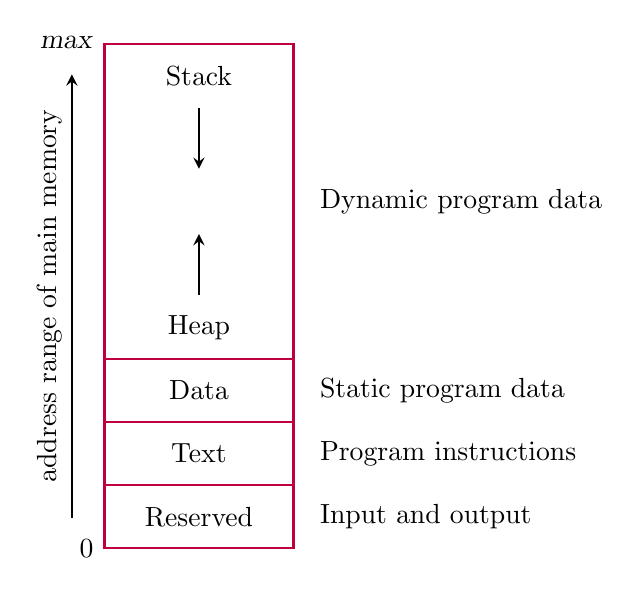
\begin{tikzpicture}[]
    \newcommand{\cellheight}[0]{8mm}
    \newcommand{\cellwidth}[0]{24mm}
    
    \tikzstyle{dedge} = [thick,->,>=stealth,draw=black]
    
    \tikzstyle{cell}=[
      rectangle,
      draw=purple,
      anchor=north,
      thick,
      minimum height=\cellheight,
      minimum width=\cellwidth,
    ]
    \tikzstyle{address}=[
      anchor=east,
    ]
    \tikzstyle{comment}=[
      anchor=west,
    ]
    
    \node[cell,minimum height=5*\cellheight] (dynsegment) at (0, -0*\cellheight) {};
    \node[cell,draw=none] (stacksegment) at (0, -0*\cellheight) {Stack};
    \node[cell,draw=none] (dotssegment) at (0, -2*\cellheight) {};
    \node[cell,draw=none] (heapsegment) at (0, -4*\cellheight) {Heap};
    \node[cell] (datasegment) at (0, -5*\cellheight) {Data};
    \node[cell] (textsegment) at (0, -6*\cellheight) {Text};
    \node[cell] (reservedsegment) at (0, -7*\cellheight) {Reserved};
    
    \node[address] () at (reservedsegment.south west) {$0$};
    \node[address] () at (dynsegment.north west) {\textsl{max}};
    
    \node[comment] () at ([xshift=2mm]dynsegment.east) {Dynamic program data};
    \node[comment] () at ([xshift=2mm]datasegment.east) {Static program data};
    \node[comment] () at ([xshift=2mm]textsegment.east) {Program instructions};
    \node[comment] () at ([xshift=2mm]reservedsegment.east) {Input and output};
    
    \draw[dedge] (stacksegment) -- (dotssegment);
    \draw[dedge] (heapsegment) -- (dotssegment);
    
    \draw[dedge] ([xshift=-4mm,yshift= 4mm]reservedsegment.south west)
              -- ([xshift=-4mm,yshift=-4mm]dynsegment.north west)
              node[midway,sloped,above] {address range of main memory}
    ;
  \end{tikzpicture}
\end{center}

  \caption{Memory model.}
  \label{fig:machine:memory}
\end{figure}

\subsection{Registers}

\subsection{Instructions}

\subsubsection{Memory Access}

\subsubsection{Arithmetic Operations}

\subsubsection{Choice}


\section{Programming Languages}
\label{sec:lang}

\begin{inspiration}{\idx{Larry Wall}{Wall, Larry}\cite{progLangJurassicPark}}
  \quoted{It might seem easy enough, but computer language design is just like a stroll in the park. Jurassic Park, that is.}
\end{inspiration}

% intro
In order to build a program, we describe \textsl{how} that program should work or \textsl{what} it should do. This is done according to the formalized rules of a \defi{programming language}. Most such languages will have high-level abstractions (compared the the assembly instructions known to the machine). They are designed in such a way that a human can reason about them. Those descriptions are stored in files and referred to as \idx{source code}{Source code}. Later on, that source code in converted into instructions and executed.

% different languages and categorization
There are many programming languages to pick from, and they each have strong and weak points. When faced with a particular problem it is important to pick a language that have relevant strong points and acceptable weak points. Many properties can be used to classify these languages. Figure \ref{fig:background:lang:categorization} focuses on two properties, namely whether there is a separate phase for compiling and whether a garbage collector is employed.

\begin{figure}[tbp]
  % inspiration: https://tex.stackexchange.com/questions/309425/how-is-it-possible-to-make-a-magic-quadrant
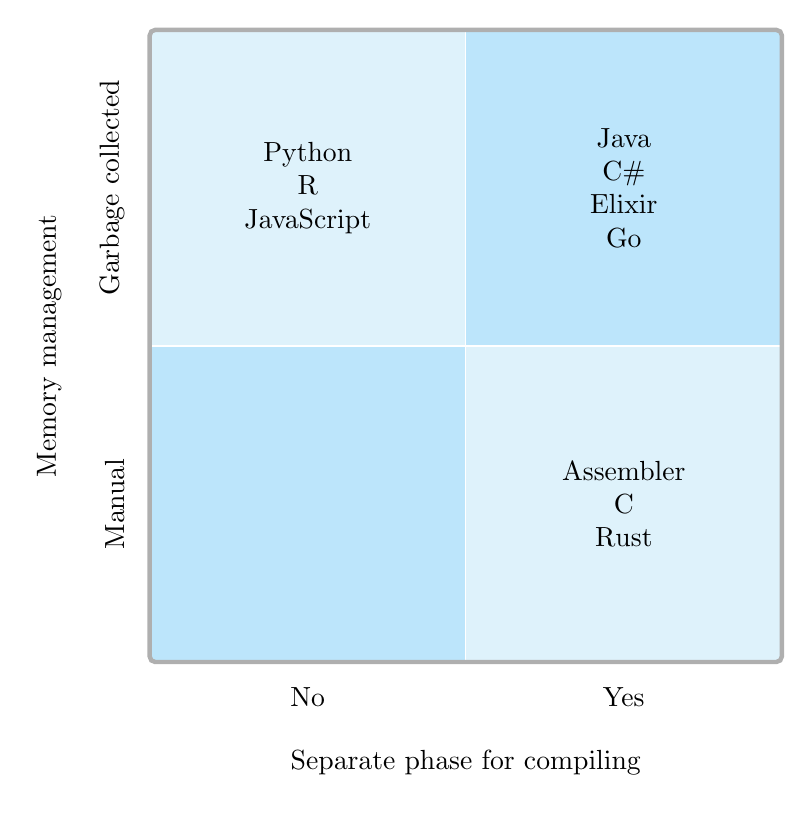
\begin{tikzpicture}[squares/.style={align=center, text width=3cm, minimum width=4cm, minimum height=4cm}]
  \node[squares,fill=lightblue] (A) at (0,0) {Python\\R\\JavaScript};
  \node[squares,fill=darkblue,anchor=west] (B) at (A.east) {Java\\\csharp\\Elixir\\Go};
  \node[squares,fill=darkblue,anchor=north] (C) at (A.south){};
  \node[squares,fill=lightblue,anchor=north] (D) at (B.south) {Assembler\\C\\Rust};
  \node[inner sep=0pt,draw=grey,ultra thick,rounded corners=2pt,fit=(A)(B)(C)(D)] {}; 
  
  \node[anchor=east,xshift=-2mm] at (A.west) {\rotatebox{90}{Garbage collected}};
  \node[anchor=east,xshift=-1cm,align=right] at (A.south west) {\rotatebox{90}{Memory management}};
  \node[anchor=east,xshift=-2mm] at (C.west) {\rotatebox{90}{Manual}};
  \node[anchor=north,yshift=-2mm] at (C.south) {No};
  \node[anchor=north,yshift=-1cm] at (C.south east) {Separate phase for compiling};
  \node[anchor=north,yshift=-2mm] at (D.south) {Yes};
\end{tikzpicture}

  \caption{Categorization of programming languages.}
  \label{fig:background:lang:categorization}
\end{figure}

% separate compilation phase
As programming languages are designed for humans to write, and the machine only understands assembly instructions, something has to \idx{compile}{Compilation} the language into these instructions. Technically, this is always a separate step, but that can be more or less obvious to the user. Some compilers will give the option of compiling the code when you try to execute the code. So, the boundary is a bit fluid. Here, we are using whether the compiled code is stored on disk after compilation as the arbiter. Languages where this is not the case are often used for tying together workflows involving many processes and files. These are called \idx{scripting languages}{Programming language!Scripting}. \csharp\ is a compiled language and not a script language (even though Microsoft likes to talk about \csharp\ scripts).

% garbage collection
Throughout the lifecycle of a process, it will need temporary chunks of memory to do its work. These chunks can be of different size and the need for this can come at varying frequency. We say that the kernel \idx{allocates}{Memory!Allocation} memory to the process on demand. This ensures that the process has exclusive access to this piece of memory and thus that no other process can interfere with its business\footnote{In reality this can be be avoided through shared segments of memory, but that is a topic way too advanced for this book.}. Once the process is done with this piece of memory it is \idx{deallocated}{Memory!Deallocation} (or \idx{freed}{Memory!Freeing}) so that it can be reclaimed by the kernel and put to use later on. This process of allocation and deallocation is manual in some languages and automatic in others. When automatic, a \idx{garbage collector}{Garbage collector} component is compiled into the running code. It essentially scans all allocations and deallocate those that are no longer in use. Again, there are pros and cons with each solution. \csharp\ is a garbage collected language.

\subsection{Parsing}

% file content
The contents of a file is a sequence of \defi{bytes}{Byte}, i.e., units that each have one of 256 possible values. When we write text, these bytes are interpreted as characters and the programs we use to open such files choose to draw each character to the right of the previous one. At \idx{line breaks}{Line break} -- represented by a specific sequence of characters -- the horizontal position is moved all the way to the left and the vertical position is moved one line height down. Some programs break lines that are too wide for your screen. But that's about it. Such a text file does not contain any information about font or text size. If you want to store such information, you have to introduce a \idx{file format}{File format} that \idx{encodes}{Encoding} such information by special \idx{markup}{Markup}. But this is not relevant for files that contain code.

% human interpretation
Files containing code are raw \idx{text files}{Text file}: A sequence of characters with line breaks. As programmers, we manipulate these files through a \idx{text editor}{Text editor}, which most often -- in addition to displaying these characters -- chooses to \idx{color}{Color}-code selected subsequences to make the text more readable for \idx{humans}{Human}. However, these colors represent an \textsl{interpretation} that the tool uses to enrich the code that is actually stored. Modifying the file and saving it will not cause the interpretation to be stored, but only the underlying code. Similarly, there are some such editors that number the lines, highlight a current line, and mark matching parentheses.

% machine interpretation
The text these files contain is called \textsl{\idx{program code}{Program code}} (or simply \textsl{code}), and we change it in much the same way as we change a written report. But when we ask the computer to \idx{execute}{Execute} our program code, it sees the file in a different way. The content is of course the same, but the \textsl{interpretation} is different: Based on some rules, the computer builds a \idx{tree}{Tree} structure of the code. This process is called \idx{parsing}{Parsing} the source code.

%% TODO: tree structure

%\subsubsection{Rules}

%% https://homepage.ruhr-uni-bochum.de/jan.holthuis/posts/using-the-latex-rail-package

%\subsubsection{Parse Trees}

%% https://tex.stackexchange.com/questions/111564/create-a-syntax-tree-with-latex


\exercises{background}{Background}


\chapter{Prereqs}

Before we get started on the subject matter, we need to install a number of programs that the remainder of the book will be referring to. You will need to use these (or similar) in the exercises. This may not seem like a particularly glorious task, but it is important to know the system in front of you and tasks like these are common for a software developer.

\section{Terminal and Shell}

\subsection{Installation}
\subsubsection{Windows}
\subsubsection{MacOS X}
\subsubsection{Debian Linux}
\subsection{Verifying Success}

\section{Text Editor}

% what is a text editor

% problem
While any text editor would do, not all are created equal. In particular, not all are equally suited for beginners. Some features help you think about the code, and understand it. Such features include \idx{syntax highlighting}{Syntax!Highlighting} (the highlighting of different parts of the code according to their role), \idx{line highlighting}{Line!Highlighting} and \idx{paranthesis highlighting}{Paranthesis!Highlighting}. Other features aim to maximize the rate of code production. Such features typically allows you to be very \say{productive} without having to think a whole lot about the code. This has a tendency to lead to \idx{absent-mindedness}{Absent-mindedness} and that is especially problematic when learning how to program. When working with the subject, you need to be present in mind and think about code. Always think about what makes it tick! Features that detracts from this are undesirable. These include anything that provides you with suggestions on how to write or rewrite your code. Any kind of \idx{autocomplete}{Autocomplete} functionality -- be it rooted in \idx{generative AI}{AI!Generative} or otherwise -- diverts your thought process from solving the problem proactively. That is bad. Other editors are very keen to suggest minor rewrites according to some set of more or less well-intended guidelines. However, these guidelines were rarely intended with novice developers in mind. In fact, then often hide complexity from the developer that is critical for the development of the novice developer.

% define subset of text editors that should be used, choose zed as first choice
So, we are looking for a text editor that has the positive aids and none of the negative aids (or at least provide easily available ways of disabling them). Seasoned developers may suggest \texttt{vi} or \texttt{emacs}, but they use their own shortcuts that have gone out of fashion. If you already use them, then there are no problems sticking to them. But everyone else should move on. Developers with deep roots in the industry will cling to \idxx{Visual Studio} (which is not portable) and have strong opinions on Visual Studio Code. Those opinions can go either way. Some companies are beginning to discard applicants who prefer \idxx{Visual Studio Code} as they have observed such developer to have a tendency to be way too reliant on the aids it provides. \idxx{Rider} is a popular option but recently they have gone all in on the problematic aids. This leaves a number of options. If you are on Linux, then you could use \texttt{gedit} or \texttt{kate}. If you are on Windows, then perhaps \texttt{notepad++} is a good option. However, the \texttt{zed}\footnote{\url{https://zed.dev}} editor is a good option, and it is available for all three major platforms. So, the following instructions will target \texttt{zed}. \texttt{zed} can be a bit finicky though, especially with regards to GPUs. So, if you are experiencing trouble, install one of the others.

\subsection{Installation}
\subsubsection{Windows}
\subsubsection{MacOS X}
\subsubsection{Debian Linux}
\subsection{Verifying Success}

\section{GIT}

\subsection{Installation}
\subsubsection{Windows}
\subsubsection{MacOS X}
\subsubsection{Debian Linux}

Git is available in the standard Debian repository. Install the client by running the following command as a \idx{privileged user}{User!Privileged}:

\begin{minted}[breaklines]{shell-session}
apt install git
\end{minted}

\subsection{Verifying Success}

At this point you should be able to run the \commandname{git} command without any parameters and get a description of how to use it.

\section{\csharp\ Development Environment}

\subsection{Installation}
\subsubsection{Windows}
\subsubsection{MacOS X}
\subsubsection{Debian Linux}
\subsection{Verifying Success}

\section{Livebook}

\subsection{Installation}
\subsubsection{Windows}
\subsubsection{MacOS X}
\subsubsection{Debian Linux}

%First we need to install the \commandname{wget} command to download \commandname{asdf}. To do so, run the following command as a privileged used:

%\begin{minted}[breaklines]{shell-session}
%apt install wget
%\end{minted}

First, install the \idx{\commandname{asdf}}{ASDF} version manager. To do so, go to \url{https://github.com/asdf-vm/asdf/releases} and download the latest version for your architecture. For version 0.16.7, that should be either \filename{asdf-v0.16.7-linux-amd64.tar.gz} or \filename{asdf-v0.16.7-linux-arm64.tar.gz}, depending on whether you have an \idx{Intel/AMD}{Processor!Intel or AMD} or an \idx{ARM}{Processor!ARM} processor. Lets assume that you downloaded the \filename{asdf-v0.16.7-linux-amd64.tar.gz} file to \filename{~/Downloads}. Then do

\begin{minted}[breaklines]{shell-session}
cd ~/bin
tar -xzf ~/Downloads/asdf-v0.16.7-linux-amd64.tar.gz
\end{minted}

Now that \commandname{asdf} is installed (and in your \idx{path}{Path}), we need to add plugins for Erlang and Elixir:

\begin{minted}[breaklines]{shell-session}
asdf plugin add erlang https://github.com/asdf-vm/asdf-erlang.git
asdf plugin add elixir https://github.com/asdf-vm/asdf-elixir.git
\end{minted}

Install \idx{Erlang}{Erlang} using \commandname{asdf}:

\begin{minted}[breaklines]{shell-session}
apt install libssl-dev
apt install unixodbc-dev
apt install libwxgtk3.2-dev libwxgtk-webview3.2-dev
asdf install erlang 27.3.2
echo export ASDF_ERLANG_VERSION=27.3.2 >> ~/.bashrc
source ~/.bashrc
\end{minted}

Install \idx{Elixir}{Elixir} using \commandname{asdf}:

\begin{minted}[breaklines]{shell-session}
asdf install elixir 1.18.3-otp-27
export ASDF_ELIXIR_VERSION=1.18.3-otp-27 >> ~/.bashrc
source ~/.bashrc
\end{minted}

This should allow you to run the Elixir REPL called \commandname{iex}. You can exit it by pressing Ctrl-C twice.

Now, lets install \idx{Livebook}{Livebook} in your home directory\footnote{You probably want to place it somewhere else according to your own organizational concept, but the instructions will assume this location.}:

\begin{minted}[breaklines]{shell-session}
cd
git clone git@github.com:livebook-dev/livebook.git
cd livebook
mix deps.get --only prod
\end{minted}

Finally, lets create a script that makes starting Livebook a breeze. For this you should come up with a password. In the instructions I use the password \say{\texttt{gazelle}}

\begin{minted}[breaklines]{shell-session}
cd ~/bin
touch start-livebook
echo \#\!/usr/bin/env bash >> start-livebook
echo export LIVEBOOK_PASSWORD=gazelle >> start-livebook
echo export MIX_ENV=prod >> start-livebook
echo cd ~/livebook >> start-livebook
echo mix phx.server >> start-livebook
chmod u+x start-livebook
\end{minted}

You should now be able to start Livebook by running:

\begin{minted}[breaklines]{shell-session}
$ start-livebook
...
[Livebook] Application running at http://localhost:8080/
\end{minted}

The first time you do this, it will take a while as the application needs to be compiled. When the last line appears, you can point a browser to the URL. If it connects and asks for a password, you have successfully installed Livebook.

\subsection{Verifying Success}


\part{Imperative Programming}
\chapter{The First Program}
\label{sec:first}

\begin{inspiration}{The Linux Kernel Module Programming Guide\cite{lkmpg20070518}}
  \quoted{When the first caveman programmer chiseled the first program on the walls of the first cave computer, it was a program to paint the string `Hello, world' in Antelope pictures. Roman programming textbooks began with the `Salut, Mundi' program. I don't know what happens to people who break with this tradition, but I think it's safer not to find out.}
\end{inspiration}

\section{Phases}

% ahead-of-time compiled language, compilation phase results in a binary that is transferable (and portable) and can be executed without the precense of the compiler
\csharp\ is an ahead-of-time compiled language. This means that program execution is a step separate from program compilation. Or, to skip the technical terms, there is a compilation phase whereby a special program known as a compiler produces a program binary by processing the program source code. This binary is transferable and (fairly) portable. This means that it can be moved to a different machine and executed without the presence of a compiler. But lets take a step back a take a look of all the involved steps.

\subsection{Project Creation}

First, lets create a directory that can host our project:

\begin{minted}[]{shell-session}
aslak@gaia:/tmp$ mkdir new_project
\end{minted}

Then, we can go to that directory and initalize a new console project:

\begin{minted}[]{shell-session}
aslak@gaia:/tmp$ mkdir new_project
aslak@gaia:/tmp$ cd new_project
aslak@gaia:/tmp/new_project$ dotnet new console
The template "Console App" was created successfully.

Processing post-creation actions...
Restoring /tmp/new_project/new_project.csproj:
  Determining projects to restore...
  Restored /tmp/new_project/new_project.csproj (in 146 ms).
Restore succeeded.
\end{minted}

So, what happened? Lets take a look at what happened in our newly created directory:

\begin{minted}[]{shell-session}
aslak@gaia:/tmp/new_project$ ls
new_project.csproj  obj  Program.cs
\end{minted}

Three files were created, and one of them is a directory:
\begin{itemize}
  \item \filename{new\_project.csproj}: This is a \say{project} file. It holds \idx{metadata}{Metadata} that tells the \commandname{dotnet} command how to build the project. The build process is the process that converts our human-readable source code to a binary that can be executed on a machine. % TODO: add an exercise for determining which version of the framework dotnet should use
  \item \filename{obj}: For now, we don't care much about this directory.
  \item \filename{Program.cs}: This is our program file. It is where we write our code. Later on we will add more files. From the perspective of the \commandname{dotnet} command, the name doesn't matter. However, as your project grows, humans will find is very confusing if certain standards are not met. We will cover these throughout the book.
\end{itemize}

\subsection{Writing}

Open the \filename{Program.cs} in your text editor and make sure the contents is as follows:

\includeCsharpFile{first/hello/Program.cs}

\subsection{Saving}

Save the file. This persists to data that was present in your computers memory under the control of your text editor to disk. That way another program can easily acces it through a valid path to the file.

\subsection{Compilation}

One such program is a compiler, and that happens to be what we need to build the program binary that is needed for execution. That compiler can be called using the \commandname{dotnet} command:

\begin{minted}[]{shell-session}
aslak@gaia:/tmp/new_project$ dotnet build
  Determining projects to restore...
  All projects are up-to-date for restore.
  new_project -> /tmp/new_project/bin/Debug/net8.0/new_project.dll

Build succeeded.
    0 Warning(s)
    0 Error(s)

Time Elapsed 00:00:05.36
\end{minted}

If we list the contents of the project directory we will see that a new \filename{bin} directory has been created for storing the binary program:

\begin{minted}[]{shell-session}
aslak@gaia:/tmp/new_project$ ls
bin  new_project.csproj  obj  Program.cs
\end{minted}

\subsection{Execution}

While we say that the compiler has produced an executable binary for us, it is not a binary that our hardware is capable of running. We need a \idx{virtual machine}{Virtual machine} for that. This is essentially a special program that simulates a different architecture. The binary we have contains \idx{Intermediate Language}{Intermediate language (IL)} (IL) bytecode, and we need a \idx{Common Language Runtime}{Common Language Runtime (CLR)} (CLR) virtual machine to execute it. Luckely, once again, the \commandname{dotnet} command gives us access to such:

\begin{minted}[]{shell-session}
aslak@gaia:/tmp/new_project$ dotnet run
Hello, World!
\end{minted}

\subsection{Big Picture}

A typical development cycle looks like figure \ref{fig:first:phases:cycle}: First a project is created, then the developer writes some code that is then compiled and executed. When writing the text editor may provide hints of errors that the developer then takes into account. The \idx{compiler}{Compiler} may give provide feedback in the form of \idx{errors}{Error} or \idx{warnings}{Warning} that need to be addressed. When executing, one might discover \idx{bugs}{Bug} that needs fixing. All of this brings us back to the writing phase.

On top of that, developers usually work on a small portion of the intended functionality. When that functionality is deemed correct -- as there are no indicators of problems in our \textsl{Write}, \textsl{Compile} and \textsl{Execute} phases -- the developer takes on an other portion and starts in the \textsl{Write} phase.

\begin{figure}[tbp]
  \begin{center}
  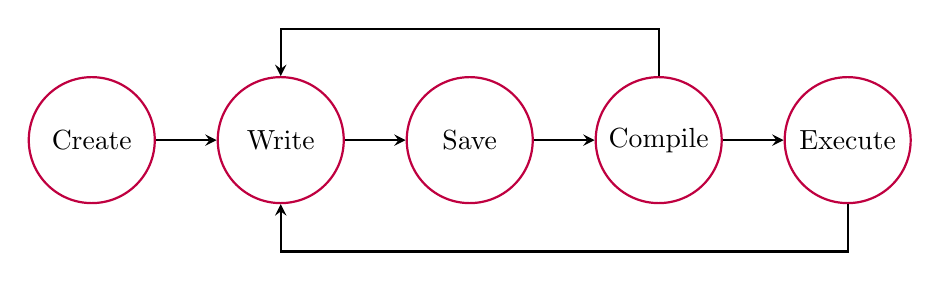
\begin{tikzpicture}[remember picture]
    \newcommand{\stepsize}{24mm}
    \tikzstyle{edge}  = [thick,>=stealth,draw=black]
    \tikzstyle{dedge} = [thick,->,>=stealth,draw=black]
    \tikzstyle{node}=[
      circle,
      draw=purple,
      anchor=center,
      thick,
      minimum size=16mm,
    ]
    
    \node[node] (nCreate) at (0*\stepsize,0) {Create};
    \node[node] (nWrite) at (1*\stepsize,0) {Write};
    \node[node] (nSave) at (2*\stepsize,0) {Save};
    \node[node] (nCompile) at (3*\stepsize,0) {Compile};
    \node[node] (nExecute) at (4*\stepsize,0) {Execute};
    
    \draw[dedge] (nCreate)--(nWrite);
    \draw[dedge] (nWrite)--(nSave);
    \draw[dedge] (nSave)--(nCompile);
    \draw[dedge] (nCompile)--(nExecute);
    \draw[dedge] (nCompile)--([yshift= 6mm]nCompile.north)-|(nWrite);
    \draw[dedge] (nExecute)--([yshift=-6mm]nExecute.south)-|(nWrite);
  \end{tikzpicture}
\end{center}

  \caption{Typical developer cycle.}
  \label{fig:first:phases:cycle}
\end{figure}

\pythonsubsection{Python}

In Python, the equivalent program looks like this:

\includePythonFile{first/hello/hello.py}

In order to execute this script, we first need to make the file \idx{executable}{File!Executable}:
\begin{minted}[]{shell-session}
aslak@gaia:/tmp/python_hello$ chmod u+x hello.py
\end{minted}

That first line of the Python source code is called a \idx{shebang}{Shebang} after the first two characters. When executing, this line uses the \filename{/bin/env} program to look up an appropriate interpreter for \filename{python3} and then feed the remaining lines to it. This is known as a \idx{dispatch mechanism}{Dispatch mechanism}. The development cycle is very similar to \csharp\ except that there is neither an initial project creation step or a separate compilation step. Running the program is done like so:

\begin{minted}[]{shell-session}
aslak@gaia:/tmp/python_hello$ ./hello.py
Hello, World!
\end{minted}

The Python interpreter has an \idx{interactive mode}{Mode!Interactive} that we can \idx{invoke}{Invoke} directly:

\begin{minted}[]{shell-session}
aslak@gaia:/tmp/python_hello$ /bin/env python3
Python 3.13.3 (main, Apr 10 2025, 21:38:51) [GCC 14.2.0] on linux
Type "help", "copyright", "credits" or "license" for more information.
>>> print("Hello, World!")
Hello, World!
>>> 
\end{minted}

On the first line we invoke the interpreter. Then, it -- exactly as our shell -- presents us with a prompt. This prompt allows us to \idx{issue}{Issue} python commands. The interactive mode is typically used for rapid experimentation.

Another way to write python code is though a \idx{notebook}{Notebook} environment. Such an environment is usually provided through a browser by a system such as \idx{Jupyter}{Jypyter}. In such an environment, code is split up into cells and these cells are laid out in a sequence. Any cell can build on the code that is introduced in previous cells and the code in these cells have easily accessible means for producing visual outputs. The workflow is essentially the same as for \csharp\ except that notebooks are usually saved automatically.

\csubsection{C}

The minimal hello world program in C looks (more or less) like this:

\includeCFile{first/hello/hello.c}

This version immediately looks a lot more complicated! So, why is that? Well, lets try to disect it \ldots

\subsubsection{Explanation}

% first line
Most \idx{general-purpose languages}{Language!General-purpose} (like \csharp, C, Python and Elixir) come with a sizeable \idx{library}{Library} of functionality. While all of this is available to you as a programmer there are downsides to having it all adirectly available all the time. To simplify grossly, it is a situation similar to finding a specific needle in a stack of slighty different needles. The first line tells C -- or rather the C preprocessor -- to include the definitions present in the \filename{stdio.h} file. This pulls in, amongst others, the \funcname{printf} function, that can print stuff to the screen for us.

% main function
Wrapping use of that \funcname{printf} function is the declaration of \funcname{main}. This is the main entry point of the program. That means that this is where the execution of the program starts. It informs the program of how many options have been passed to it (through \varname{argc}) and what those options are (through \varname{argv}). This is \idx{kernels}{Kernel} primary means of informing a program of what inputs it should operate on. The \typename{int} before \funcname{main} indicates that the program evaluates to an integer value. It is convention that a zero indicates success and a non-zero value functions an an \idx{error code}{Error code}. As this program doesn't explicitly return such a number, it will default to zero.

It is important to point out that \csharp\ supports a very similar program structure. After all, this is how the kernel passes options to a program. Any language that supports such options will have something similar. It is typically in a \idx{\funcname{main} function}{Function!Main}. But sometimes it is implicit or has to be actively \idx{imported}{Importing}. That is not likely to mean much to you at this point, and that is okay.

\subsubsection{Workflow}

In order to compile the code to an executable binary we need to invoke a compiler. Lets use the \commandname{clang} compiler and explicitly name the file that should hold the resulting binary:

\begin{minted}[]{shell-session}
aslak@gaia:/tmp/c_hello$ clang hello.c -o hello
\end{minted}

One key difference, compared to \csharp, is that C compiles to a \defi{native binary}{Binary!Native}. That is a binary that follows a format that is directly compatible with the processor architecture of your computer. We notice this when executing the code. With \csharp we used \commandname{dotnet} to essentially simulate a virtual machine that was capable of interpreting the intermediate language binary. This manifested as a command that began with \commandname{dotnet}.

The \commandname{dotnet} program that is then invoked is another example of a native binary. So, we can invoke the binary that we have built from our C code in exactly the same way. However, unlike \commandname{dotnet}, our binary is not in the \idx{path}{Path}. That means that we need an \idx{explicit path}{Path!Explicit} to it. That is accomplished by prefacing it with \filename{./}, like so:

\begin{minted}[]{shell-session}
aslak@gaia:/tmp/c_hello$ ./hello
Hello, World!
\end{minted}

\elixirsubsection{Elixir}

Elixir code can be executed through an interpreter (like Python), it can be worked on through a notebook system (like Python) and it can be executed on a virtual machine (like \csharp). This virtual machine is called \idx{BEAM}{BEAM}. Unlike that for \csharp, it is a \idx{distributed}{Virtual machine!Distributed} virtual machine. The hello world program looks different depending on whether a separate compilation phase is used or the code is interpreted. For the interpreter, the code looks like this:

\includeElixirFile{first/hello/hello.exs}

% mix creating new project

% interpreter with access to new project

% interpreter hooking into other virtual machine

% livebook

\subsection{Summary}

% ref to fig, what does that mean? Is it better to have more boxes checked? Why and why not?
The covered languages support for \idx{execution models}{Execution model} is summarized in figure \ref{fig:first:phases:summary}. C and \csharp\ only support a single model each, while Elixir supports 5 (or 3 with variations). Does that mean that Elixir is a superior language? No, certainly not. But it does mean that you have more options as to how you execute Elixir code. Sometimes support for specific execution models matter, but often it does not.

\begin{figure}[tbp]
  \begin{center}
  \begin{tabular}{ccccl}
    \rotatebox{90}{\textbf{C}} & \rotatebox{90}{\textbf{\csharp}} & \rotatebox{90}{\textbf{Python}} & \rotatebox{90}{\textbf{Elixir}} & \textbf{Execution model} \\
    $\times$ & & & & Compile and execute directly on hardware \\
    & $\times$ & & $\times$ & Compile and execute in VM \\
    & & $\times$ & $\times$ & Script \\
    & & $\times$ & $\times$ & REPL \\
    & & $\times$ & $\times$ & Notebook \\
    & & & $\times$ & Script attached to running VM \\
    & & & $\times$ & REPL attached to running VM \\
    & & & $\times$ & Notebook attached to running VM \\
  \end{tabular}
\end{center}

  \caption{Summary of execution models of various programming languages.}
  \label{fig:first:phases:summary}
\end{figure}

% tradeoffs
It is also important to point out that the design of a programming language is riddled with \idx{tradeoffs}{Tradeoff}, and these are often resolved in very different ways. That results in some set of qualities, of which the supported set of execution models are found. As a developer, it will be your job to decide which combination of qualities are needed to maximize \idx{value}{Value} for a given project, and based on that choose a language.

\section{Strings}
\label{sec:string}




\chapter{Primitive Types}

\section{Numbers}

% everything is a number, not always obvious, classes of numbers, the simples calls is integers
All values that we may want to work with in a computer are, one way or the other, \idx{numbers}{Number}. This fact may not always be obvious, but it will be quite a while before you encounter such examples. From public school and highschool, we know these classes of numbers:
\begin{itemize}
  \descitem{The \idx{natural numbers}{Numbers!Natural}} ($\mathbb{N}$) These are the non-negative numbers that can be written without a decimal point\footnote{There are two definitions of natural numbers. The other definition is that they are the positive numbers that can be written without a decimal point. That is to say, without zero. As this definition is generally less applicable in computers, we stick to the first definition.}.
  \descitem{The \idx{integers}{Numbers!Integer}} ($\mathbb{Z}$) These are all the natural numbers (according to the first definition) along with the negative versions of the natural numbers (according to the second definition). That definition juggling is to make sure that we don't have a negative zero.
  \descitem{The \idx{real numbers}{Numbers!Real}} ($\mathbb{R}$) These are all the numbers that can be placed on a line between $-\infty$ and $\infty$. We often refer to these as floating point numbers.
  \descitem{The \idx{rational numbers}{Numbers!Rational}} ($\mathbb{Q}$) These are then numbers that can be written as the fraction $m/n$ where $m \in \mathbb{Z}$ and $m \in \mathbb{N}$.
  \descitem{The \idx{irrational numbers}{Numbers!Irrational}} ($\mathbb{P}$) These are numbers that belong to $\mathbb{R}$ but not $\mathbb{Q}$. This is where $\pi$ and $e$ belong.
\end{itemize}
Computers typically works with other classes of numbers. In the following sections, we will explore the most commonly used ones. Common to these is that they are all \idx{represented in binary}{Representation!Binary} numbers. That is, using the \idx{base-2}{Base 2} digits. We are used to working with \idx{base-10}{Base 10} where numbers are digits between zero and nine. In base-2, the numbers are made up of digits between zero and one (i.e., \texttt{0} or \texttt{1}). Such a digit is called a \defi{bit}{Bit}, and a sequence of eight bits is referred to as a \defi{byte}{Byte}. The plural forms of the singular bit and byte is bits and bytes. Bits are, by the way, the \idx{SI unit}{SI unit} of information, in the same way as meter is the SI unit of distance. Accordingly, we measure \idx{information}{Information} in bits.

\section{Integers}

\subsection{Operations}

% basic operations
All general purpose languages support the four basic \idx{arithmetic operators}{Operation!Arithmetic} for addition, subtraction, multiplication and division of integers. The tree first of these will guarantee an integral result. For instance, if you add two integers, you will get an integer. The \textsl{size} of this integer may be affected though. But more on that in section \ref{primitives:int:representation}.

% that division thing
That rule, about the result of an operation resuling in an integral value does not hold for the \idx{division}{Operation!Division} operation though. Mathematically, the result \textsl{may} be integral, but generally speaking there is no guarantee, and more often than not it is simply not the case. Most programming languages supports two types of division; namely \idx{integer division}{Operation!Division!Integer} and \idx{floating-point division}{Operation!Division!Floating-point}. The result of a floating-point division is a floating-point number as introduced in section \ref{primitives:float}. The result of an integer division is an integer.

% remainder vs modulo
This operation is tightly coupled to both the \idx{remainder}{Remainder} and the \idx{modulo}{Modulo} operations. The difference between these is how they handle negative numbers.

% TODO: Figure of remainder vs modulo

\subsection{Representation}
\label{primitives:int:representation}

% typical representation

% signedness

\csharpsubsection{\csharp}

\begin{syntaxsegment}
  Test
\end{syntaxsegment}

\begin{syntaxfloat}
  \begin{syntax}{expr}
    \node[nonterminal] (ruleIa)  at (4cm,\SyntaxRow{0}) {expr};
    \node[terminal]    (ruleIb)  at (6cm,\SyntaxRow{0}) {+};
    \node[nonterminal] (ruleIc)  at (8cm,\SyntaxRow{0}) {expr};
    \node[nonterminal] (ruleIIa) at (4cm,\SyntaxRow{1}) {expr};
    \node[terminal]    (ruleIIb) at (6cm,\SyntaxRow{1}) {-};
    \node[nonterminal] (ruleIIc) at (8cm,\SyntaxRow{1}) {expr};
    
    \draw[path] (begin)--(ruleIa)--(ruleIb)--(ruleIc)--(end);
    \draw[path] (begin) to[-|-] (ruleIIa)--(ruleIIb)--(ruleIIc) to[-|-] (end);
  \end{syntax}
  \caption{Expressions of arithmetic operators}
\end{syntaxfloat}

% integer types available

\begin{figure}[tbp]
  \begin{center}
  \begin{tabular}{rccl}
    \emph{Size} & \emph{Unsigned Type} & \emph{Signed Type} & \emph{Comment} \\
     8 bits & \typename{byte} & \typename{sbyte} & \\
    16 bits & \typename{ushort} & \typename{short} & \\
    32 bits & \typename{uint} & \typename{int} & \\
    64 bits & \typename{ulong} & \typename{long} & \\
    1 word & \typename{nuint} & \typename{nint} & Do not use \\
  \end{tabular}
\end{center}

  \caption{Integer types available in \csharp.}
  \label{fig:prim:int:csharp:types}
\end{figure}

% what is the result of int32+int32? what is an overflow?

\elixirsubsection{Elixir}

% arbitrary sizes: pros
In Elixir, there is only one integer type and that has an \idx{arbitrary size}{Arbitrary size}. As long as an integral value fits in memory, an Elixir integer can hold it. The value is not in having integers that each take up 90\% of your \idx{primary memory}{Memory!Primary}. It is very rare that we have a need for integers beyond 128 bits or even 64 bits. But when we work with \idx{fixed size}{Fixed size} integers, we always have to be aware of that hard limit. In Elixir, we don't have to: If we somehow end up with a number needing 7000 bits, then that is what gets allocated. We don't have to worry.

% and cons, why the tradeoff was resolved in this way
Elixir code, still runs on the same hardware though. This hardware does not have instructions capable of operating on 7000 bit integers. So, instead of an integer operation being a single \idx{instruction}{Instruction}, it is an \idx{algorithm}{Algorithm} in itself. This is significantly slower. Elixir is designed for network intensive tasks, and these are even slower. So, for the tasks where one would choose Elixir, it basically doesn't matter. And that is why the designers of that language has made that choice.

\section{Floating Point Numbers}
\label{primitives:float}

\subsection{Operations}
\subsection{Representation}
\csharpsubsection{\csharp}
\elixirsubsection{Elixir}

\section{Truth Values}

% what do they represent

\subsection{Operations on Nontruthy Values}

Any valid comparison between two nontruthy values will yield a truthy value. For instance, if we ask \quoted{is 42 equal to 56?} then the resulting value is \valuename{false} but if we ask \quoted{is 1 less than or equal to 2?} then the resulting value is \valuename{true}.

\begin{figure}[tbp]
  \begin{center}
  \begin{tabular}{cl}
    $a$ \texttt{==} $b$ & True if $a$ is the same as $b$ \\
    $a$ \texttt{!=} $b$ & True if $a$ is different from $b$ \\
    $a$ \texttt{<} $b$ & True if $a$ is less than $b$ \\
    $a$ \texttt{<=} $b$ & True if $a$ is less than or equal to $b$ \\
    $a$ \texttt{>} $b$ & True if $a$ is greater than $b$ \\
    $a$ \texttt{>=} $b$ & True if $a$ is greater than or equal to $b$ \\
  \end{tabular}
\end{center}

  \caption{Comparison operators.}
  \label{fig:prim:bool:comparison}
\end{figure}

\subsection{Operations on Truth Values}

\begin{figure}[tbp]
  \input{figs/prim_bool_and.tex}
  \caption{Truth table for the boolean operations.}
  \label{fig:prim:bool:and}
\end{figure}

% TODO: De Morgan's law

\subsection{Representation}

% technically a bit, but typically (mostly unless in array form) a byte or word

\csharpsubsection{\csharp}

\elixirsubsection{Elixir}

\csubsection{C}

% low-level language
\idx{C}{Language!C} is a simple \idx{low-level language}{Language!Low-level}. That means that it mirrors the fundamental properties of the underlying harware and adds some highly convenient abstractions. These abstractions are chosen is such a way that they essentially can be delivered without a performance overhead.

% consequence: a boolean is a register
\idxx{Machine code} does not have a boolean type. Instead \idx{register}{Register} values that are represented using all zeroes in binary are \textsl{false} and every other value is \textsl{true}. That means -- in terms of integers -- that zero is \textsl{false} and non-zero is \textsl{true}. % TODO: Explain the !!42 == 1 situation, word for reference/strong true values, implicit konvertering til bool i condition af en if

% consequence: a bool is an integer and can thus be used in an integer expression
A consequence of this is that C doesn't have a notion of a \idx{boolean}{Boolean}. Instead, integers are used: A boolean is an interpretation of an integer, and can thus be used in an integer expression. Typically, this will make absolutely no difference. Proponents of \csharp\ will point out that booleans and integers are fundamentally different notions and should thus be treated differently. Proponents of C will point out that this allows them to write code such as this:

% TODO: Example

% explanation: why is this clever (no branches gives execution speed, and it is still readable)

\section{Variables}
\csharpsubsection{\csharp}
\elixirsubsection{Elixir}

\section{Parsing}
\subsection{Operator Precedence}
\subsection{Operator Associativity}

\exercises{primitives}{Primitive Types}


\chapter{Flow Control}

% motivation
So far, we have worked with a strict sequence of \idx{statements}{Statement}. All of these statements are evaluated, in \idx{order}{Order}. This is a quality that we will often come to rely on. But it is not expressive enough. 

\begin{figure}[tbp]
  \begin{center}
  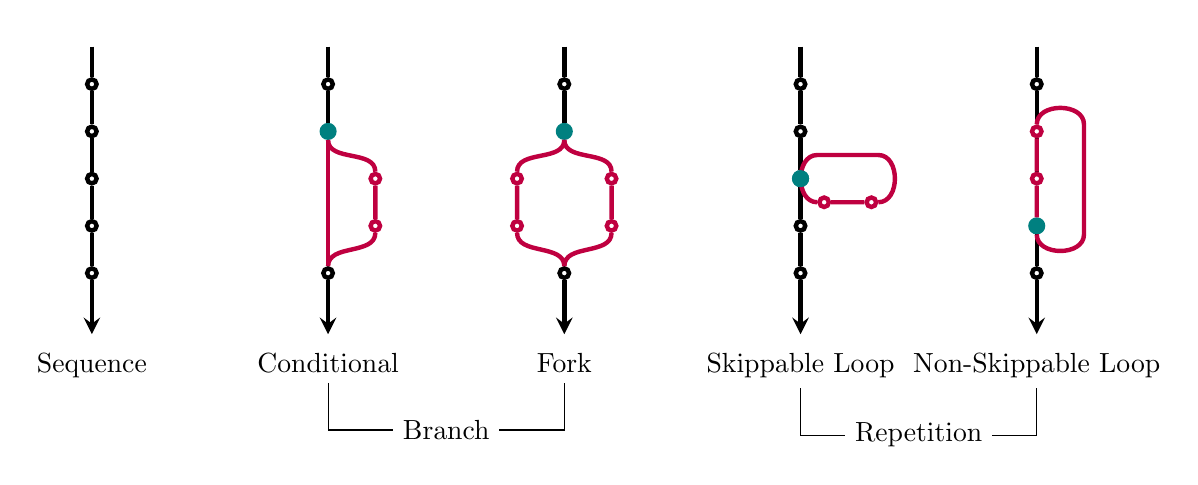
\begin{tikzpicture}[]
    \newcommand{\spacing}[0]{6mm}
    \newcommand{\absspacing}[0]{30mm}
    \newcommand{\seqX}[0]{ 0*\absspacing}
    \newcommand{\condX}[0]{1*\absspacing}
    \newcommand{\forkX}[0]{2*\absspacing}
    \newcommand{\whileX}[0]{3*\absspacing}
    \newcommand{\dowhileX}[0]{4*\absspacing}
    
    \tikzstyle{endpoint} = []
    \tikzstyle{stmt} = [circle,ultra thick,inner sep=0pt,minimum size=1.2mm,fill=none,draw=black]
    \tikzstyle{arrow} = [thick,->,>=stealth, draw=black]
    \tikzstyle{flow} = [arrow,ultra thick]
    \tikzstyle{label} = [anchor=north]
    \tikzstyle{subtype} = [draw=black]
    \tikzstyle{choice} = [draw=teal,fill=teal,minimum size=1.6mm]
    
    \coordinate (seqAnchor)  at (\seqX ,0);
    \coordinate (condAnchor) at (\condX,0);
    \coordinate (forkAnchor) at (\forkX,0);
    \coordinate (whileAnchor) at (\whileX,0);
    \coordinate (dowhileAnchor) at (\dowhileX,0);
    
    % sequence
    {
      \node[endpoint] (seqBegin) at ([yshift=0*\spacing]seqAnchor) {};
      \node[stmt] (seqA) at ([yshift=-1*\spacing]seqAnchor) {};
      \node[stmt] (seqB) at ([yshift=-2*\spacing]seqAnchor) {};
      \node[stmt] (seqC) at ([yshift=-3*\spacing]seqAnchor) {};
      \node[stmt] (seqD) at ([yshift=-4*\spacing]seqAnchor) {};
      \node[stmt] (seqE) at ([yshift=-5*\spacing]seqAnchor) {};
      \node[endpoint] (seqEnd) at ([yshift=-6.5*\spacing]seqAnchor) {};
      \node[label] () at ([yshift=0*\spacing]seqEnd) {Sequence};
      
      \path[flow] (seqBegin)
               -- (seqA)
               -- (seqB)
               -- (seqC)
               -- (seqD)
               -- (seqE)
               -- (seqEnd)
      ;
    }
    
    % conditional
    {
      \node[endpoint] (condBegin) at ([yshift=0*\spacing]condAnchor) {};
      \node[stmt] (condA) at ([yshift=-1*\spacing]condAnchor) {};
      \node[stmt,choice] (condB) at ([yshift=-2*\spacing]condAnchor) {};
      \node[stmt,draw=purple] (condC) at ([yshift=-3*\spacing,xshift=\spacing]condAnchor) {};
      \node[stmt,draw=purple] (condD) at ([yshift=-4*\spacing,xshift=\spacing]condAnchor) {};
      \node[stmt] (condE) at ([yshift=-5*\spacing]condAnchor) {};
      \node[endpoint] (condEnd) at ([yshift=-6.5*\spacing]condAnchor) {};
      \node[label] (cond) at ([yshift=0*\spacing]condEnd) {Conditional};
      
      \path[flow,-] (condBegin)
               -- (condA)
               -- (condB)
      ;
      \path[flow,-,draw=purple] (condB)
               -- (condE)
      ;
      \path[flow,-,draw=purple] (condB)
               to [out=270,in=90] (condC)
               -- (condD)
               to [out=270,in=90]  (condE)
      ;
      \path[flow] (condE)
               -- (condEnd)
      ;
    }
    
    % fork
    {
      \node[endpoint] (forkBegin) at ([yshift=0*\spacing]forkAnchor) {};
      \node[stmt] (forkA) at ([yshift=-1*\spacing]forkAnchor) {};
      \node[stmt,choice] (forkB) at ([yshift=-2*\spacing]forkAnchor) {};
      \node[stmt,draw=purple] (forkCtrue) at ([yshift=-3*\spacing,xshift=-\spacing]forkAnchor) {};
      \node[stmt,draw=purple] (forkDtrue) at ([yshift=-4*\spacing,xshift=-\spacing]forkAnchor) {};
      \node[stmt,draw=purple] (forkCfalse) at ([yshift=-3*\spacing,xshift=\spacing]forkAnchor) {};
      \node[stmt,draw=purple] (forkDfalse) at ([yshift=-4*\spacing,xshift=\spacing]forkAnchor) {};
      \node[stmt] (forkE) at ([yshift=-5*\spacing]forkAnchor) {};
      \node[endpoint] (forkEnd) at ([yshift=-6.5*\spacing]forkAnchor) {};
      \node[label] (fork) at ([yshift=0*\spacing]forkEnd) {Fork};
      
      \path[flow,-] (forkBegin)
               -- (forkA)
               -- (forkB)
      ;
      \path[flow,-,draw=purple] (forkB)
               to [out=270,in=90] (forkCtrue)
               -- (forkDtrue)
               to [out=270,in=90] (forkE)
      ;
      \path[flow,-,draw=purple] (forkB)
               to [out=270,in=90] (forkCfalse)
               -- (forkDfalse)
               to [out=270,in=90] (forkE)
      ;
      \path[flow] (forkE)
               -- (forkEnd)
      ;
    }
    
%    % while loop
%    {
%      \node[endpoint] (whileBegin) at ([yshift=0*\spacing]whileAnchor) {};
%      \node[stmt] (whileA) at ([yshift=-1*\spacing]whileAnchor) {};
%      \node[stmt,choice] (whileB) at ([yshift=-2*\spacing]whileAnchor) {};
%      \node[stmt,draw=purple] (whileC) at ([yshift=-3*\spacing]whileAnchor) {};
%      \node[stmt,draw=purple] (whileD) at ([yshift=-4*\spacing]whileAnchor) {};
%      \node[stmt] (whileE) at ([yshift=-5*\spacing,xshift=-\spacing]whileAnchor) {};
%      \node[stmt] (whileF) at ([yshift=-6*\spacing,xshift=-\spacing]whileAnchor) {};
%      \node[endpoint] (whileEnd) at ([yshift=-7.5*\spacing,xshift=-\spacing]whileAnchor) {};
%      \node[label] (while) at ([yshift=0*\spacing]whileEnd) {Skippable Loop};
%      
%      \path[flow] (whileBegin)
%               -- (whileA)
%               -- (whileB)
%               to [out=270,in=90] ([yshift=-1*\spacing,xshift=-1*\spacing]whileB)
%               -- (whileE)
%               -- (whileF)
%               -- (whileEnd)
%      ;
%      \path[flow,-,draw=purple] (whileB)
%               -- (whileC)
%               -- (whileD)
%               to [out=270,in=270] ([xshift=1*\spacing]whileD)
%               -- ([xshift=1*\spacing]whileB.center)
%               to [out=90,in=90] (whileB)
%      ;
%    }
    
    % while loop
    {
      \node[endpoint] (whileBegin) at ([yshift=0*\spacing]whileAnchor) {};
      \node[stmt] (whileA) at ([yshift=-1*\spacing]whileAnchor) {};
      \node[stmt] (whileB) at ([yshift=-2*\spacing]whileAnchor) {};
      \node[stmt,choice] (whileC) at ([yshift=-3*\spacing]whileAnchor) {};
      \node[stmt,draw=purple] (whileD) at ([yshift=-3.5*\spacing,xshift=0.5*\spacing]whileAnchor) {};
      \node[stmt,draw=purple] (whileE) at ([yshift=-3.5*\spacing,xshift=1.5*\spacing]whileAnchor) {};
      \node[stmt] (whileF) at ([yshift=-4*\spacing]whileAnchor) {};
      \node[stmt] (whileG) at ([yshift=-5*\spacing]whileAnchor) {};
      \node[endpoint] (whileEnd) at ([yshift=-6.5*\spacing]whileAnchor) {};
      \node[label] (while) at ([yshift=0*\spacing]whileEnd) {Skippable Loop};
      
      \path[flow] (whileBegin)
               -- (whileA)
               -- (whileB)
               -- (whileC)
               -- (whileF)
               -- (whileG)
               -- (whileEnd)
      ;
      \path[flow,-,draw=purple](whileD)
               -- (whileE)
               to [out=0,in=0,looseness=1.2] ([yshift=1*\spacing]whileE.east)
               -- ([yshift=1*\spacing]whileD.west)
               to [out=180,in=180,looseness=1.2] (whileD.west)
      ;
      
      % TODO: this is a hack to make this node appear on top of the loop path
      \node[stmt,choice] (whileC) at ([yshift=-3*\spacing]whileAnchor) {};
    }
    
    % do-while loop
    {
      \node[endpoint] (dowhileBegin) at ([yshift=0*\spacing]dowhileAnchor) {};
      \node[stmt] (dowhileA) at ([yshift=-1*\spacing]dowhileAnchor) {};
      \node[stmt,draw=purple] (dowhileB) at ([yshift=-2*\spacing]dowhileAnchor) {};
      \node[stmt,draw=purple] (dowhileC) at ([yshift=-3*\spacing]dowhileAnchor) {};
      \node[stmt,choice] (dowhileD) at ([yshift=-4*\spacing]dowhileAnchor) {};
      \node[stmt] (dowhileE) at ([yshift=-5*\spacing]dowhileAnchor) {};
      \node[endpoint] (dowhileEnd) at ([yshift=-6.5*\spacing]dowhileAnchor) {};
      \node[label] (dowhile) at ([yshift=0*\spacing]dowhileEnd) {Non-Skippable Loop};
      
      \path[flow] (dowhileBegin)
               -- (dowhileA)
               -- (dowhileB)
               -- (dowhileC)
               -- (dowhileD)
               -- (dowhileE)
               -- (dowhileEnd)
      ;
      \path[flow,-,draw=purple] (dowhileB)
               -- (dowhileC)
               -- (dowhileD)
               to [out=270,in=270,looseness=1.2] ([xshift=1*\spacing]dowhileD.south)
               -- ([xshift=1*\spacing]dowhileB.north)
               to [out=90,in=90,looseness=1.2] (dowhileB)
      ;
    }
    
    % branch
    \node[label] (branch) at ([yshift=-1*\spacing] $(cond)!0.5!(fork)$) {Branch};
    \path[subtype] (cond) |- (branch) -| (fork);
    
    % loop
    \node[label] (loop) at ([yshift=-1*\spacing] $(while)!0.5!(dowhile)$) {Repetition};
    \path[subtype] (while) |- (loop) -| (dowhile);
  \end{tikzpicture}
\end{center}

  \caption{Basic flow abstractions.}
  \label{fig:flow:types}
\end{figure}

\section{Choices in Logic}
\label{sec:flow:branch}

Hello

\subsection{\keywordname{if} and \keywordname{else}}
\subsection{\keywordname{unless}}
\subsection{Chaining Branches}
\subsection{\keywordname{switch} and \keywordname{case}}

\csharpsubsection{\csharp}

\begin{syntaxfloat}
  \section{Choices in Logic}
\label{sec:flow:branch}

Hello

\subsection{\keywordname{if} and \keywordname{else}}
\subsection{\keywordname{unless}}
\subsection{Chaining Branches}
\subsection{\keywordname{switch} and \keywordname{case}}

\csharpsubsection{\csharp}

\begin{syntaxfloat}
  \input{syntax/flow_branch.tex}
  \caption{Statements for branching}
  \label{syntax:flow:branch}
\end{syntaxfloat}

\elixirsubsection{Elixir}
hello

\subsection{Blocks}

\subsubsection{Dangling Else}
\label{sec:flow:branch:danglingelse}

\csharpsubsection{\csharp}

\begin{syntaxfloat}
  \input{syntax/flow_block.tex}
  \caption{Block statements}
  \label{syntax:flow:block}
\end{syntaxfloat}


  \caption{Statements for branching}
  \label{syntax:flow:branch}
\end{syntaxfloat}

\elixirsubsection{Elixir}
hello

\subsection{Blocks}

\subsubsection{Dangling Else}
\label{sec:flow:branch:danglingelse}

\csharpsubsection{\csharp}

\begin{syntaxfloat}
  \begin{syntax}{stmt}
  \SyntaxWestSplit{MainWest}
  \SyntaxEastSplit{MainEast}
  
  \node[sequence] () at ([yshift=0*\syntaxruledist]$(begin)!0.5!(end)$) {
    \node[terminal]    (ruleIa) {\{};
    &
    \node[nonterminal] (ruleIb) {stmts};
    &
    \node[terminal]    (ruleIc) {\}};
    \\
  };
  
  \draw[path] (begin)--(ruleIa)--(ruleIb)--(ruleIc)--(end);
\end{syntax}

  \caption{Block statements}
  \label{syntax:flow:block}
\end{syntaxfloat}


\chapter{Repetition}
\label{sec:flow:repetition}

Hello


\exercises{flow}{Flow Control}

\chapter{Basic Datastructures}

\section{Sequences in Data}

\subsection{Arrays}

\subsubsection{Multidimensiontal Arrays}

\subsection{Linked Lists}

% head and tail

\subsection{Doubly Linked Lists}

\subsection{Looping Sequences}

\subsection{Dimensions}

\section{Structured Data}

\subsection{Colors}

\subsection{Point Example}

\section{Enumerations}

\subsection{State Machines}

\subsection{String Parsing Example}


\chapter{Code Reuse}

Hello

\section{Concrete Implementations}

\csharpsubsection{\csharp}

\begin{syntaxfloat}
  \begin{syntax}[[xshift=20mm]concept.west]{params}
  \SyntaxWestSplit{MainWest}
  \SyntaxEastSplit{MainEast}
  
  \node[sequence,column sep=1.5cm] () at ([yshift=-0*\syntaxruledist]$(begin)!0.5!(end)$) {
    \node[nonterminal] (ruleIa) {type};
    &
    \node[terminal]    (ruleIb) {name};
    \\
  };
  
  \node[sequence,column sep=1.0cm] () at ([yshift=1*\syntaxruledist]$(ruleIa)!0.5!(ruleIb)$) {
    \node[terminal]    (ruleIIa) {,};
    \\
  };
  
  \draw[path] (begin)--(ruleIa)--(ruleIb)--(end);
  \draw[path] (ruleIb)
            -|([xshift= 0.75*\syntaxruledist,yshift=0.4*\syntaxruledist]ruleIb.east)
            |-(                            [yshift=0.0*\syntaxruledist]ruleIIa)
            -|([xshift=-0.75*\syntaxruledist,yshift=0.4*\syntaxruledist]ruleIa.west)
            |-(ruleIa);
  \draw[path] (begin)
            -|([xshift=-1.5*\syntaxruledist,yshift=-0.5*\syntaxruledist]ruleIa.west)
            |-(                            [yshift=-1.0*\syntaxruledist]ruleIa.center)
            -|([xshift= 1.5*\syntaxruledist,yshift=-0.5*\syntaxruledist]ruleIb.east)
            |-(end);
\end{syntax}

\begin{syntax}[[xshift=20mm]concept.west]{fun-def}
  \SyntaxWestSplit{MainWest}
  \SyntaxEastSplit{MainEast}
  
  \node[sequence,column sep=1.2cm] () at ([yshift=-0*\syntaxruledist]$(begin)!0.5!(end)$) {
    \node[nonterminal] (ruleIa) {type};
    &
    \node[terminal]    (ruleIb) {name};
    &
    \node[terminal]    (ruleIc) {(};
    &
    \node[nonterminal] (ruleId) {params};
    &
    \node[terminal]    (ruleIe) {)};
    &
    \node[terminal]    (ruleIf) {stmt};
    \\
  };
  
  \draw[path] (begin)--(ruleIa)--(ruleIb)--(ruleIc)--(ruleId)--(ruleIe)--(ruleIf)--(end);
\end{syntax}

\begin{syntax}[[xshift=20mm]concept.west]{args}
  \SyntaxWestSplit{MainWest}
  \SyntaxEastSplit{MainEast}
  
  \node[sequence,column sep=1.5cm] () at ([yshift=-0*\syntaxruledist]$(begin)!0.5!(end)$) {
    \node[nonterminal] (ruleIa) {expr};
    \\
  };
  
  \node[sequence,column sep=1.0cm] () at ([yshift=1*\syntaxruledist]ruleIa) {
    \node[terminal]    (ruleIIa) {,};
    \\
  };
  
  \draw[path] (begin)--(ruleIa)--(end);
  \draw[path] (ruleIa)
            -|([xshift= 0.75*\syntaxruledist,yshift=0.4*\syntaxruledist]ruleIa.east)
            |-(                            [yshift=0.0*\syntaxruledist]ruleIIa)
            -|([xshift=-0.75*\syntaxruledist,yshift=0.4*\syntaxruledist]ruleIa.west)
            |-(ruleIa);
  \draw[path] (begin)
            -|([xshift=-1.5*\syntaxruledist,yshift=-0.5*\syntaxruledist]ruleIa.west)
            |-(                            [yshift=-1.0*\syntaxruledist]ruleIa.center)
            -|([xshift= 1.5*\syntaxruledist,yshift=-0.5*\syntaxruledist]ruleIa.east)
            |-(end);
\end{syntax}

\begin{syntax}[[xshift=20mm]concept.west]{fun-call}
  \SyntaxWestSplit{MainWest}
  \SyntaxEastSplit{MainEast}
  
  \node[sequence,column sep=1.5cm] () at ([yshift=-0*\syntaxruledist]$(begin)!0.5!(end)$) {
    \node[terminal]    (ruleIa) {name};
    &
    \node[terminal]    (ruleIb) {(};
    &
    \node[nonterminal] (ruleIc) {args};
    &
    \node[terminal]    (ruleId) {)};
    \\
  };
  
  \draw[path] (begin)--(ruleIa)--(ruleIb)--(ruleIc)--(ruleId)--(end);
\end{syntax}

\begin{syntax}[[xshift=20mm]concept.west]{expr}
  \SyntaxWestSplit{MainWest}
  \SyntaxEastSplit{MainEast}
  
  \node[sequence,column sep=1.5cm] () at ([yshift=-0*\syntaxruledist]$(begin)!0.5!(end)$) {
    \node[nonterminal] (ruleIa) {fun-call};
    \\
  };
  
  \draw[path] (begin)--(ruleIa)--(end);
\end{syntax}

\begin{syntax}[[xshift=20mm]concept.west]{stmt}
  \SyntaxWestSplit{MainWest}
  \SyntaxEastSplit{MainEast}
  
  \node[sequence,column sep=1.5cm] () at ([yshift=-0*\syntaxruledist]$(begin)!0.5!(end)$) {
    \node[nonterminal] (ruleIa) {fun-def};
    \\
  };
  
  \node[sequence,column sep=1.5cm] () at ([yshift=-1*\syntaxruledist]$(begin)!0.5!(end)$) {
    \node[nonterminal] (ruleIIa) {fun-call};
    &
    \node[terminal]    (ruleIIb) {;};
    \\
  };
  
  \draw[path] (begin)--(ruleIa)--(end);
  \draw[path] (begin)
            -|([xshift=-1.5*\syntaxruledist,yshift=0.5*\syntaxruledist]ruleIIa.west)
            |-(                                                         ruleIIa)
            --(                                                         ruleIIb)
            -|([xshift= 1.5*\syntaxruledist,yshift=0.5*\syntaxruledist]ruleIIb.east)
            |-(end);
\end{syntax}


  \caption{Functions.}
  \label{syntax:fun}
\end{syntaxfloat}

\pythonsubsection{Python}

\elixirsubsection{Elixir}


\chapter{Exceptions}

Hello


\begin{syntaxfloat}
  \begin{syntax}[[xshift=22mm]concept.west]{stmt}
  \SyntaxWestSplit{MainWest}
  \SyntaxEastSplit{MainEast}
  
  \draw[path] (begin)--(end);
\end{syntax}

\begin{syntax}[[xshift=22mm]concept.west]{catch}
  \SyntaxWestSplit{MainWest}
  \SyntaxEastSplit{MainEast}
  
  \draw[path] (begin)--(end);
\end{syntax}

\begin{syntax}[[xshift=22mm]concept.west]{finally}
  \SyntaxWestSplit{MainWest}
  \SyntaxEastSplit{MainEast}
  
  \draw[path] (begin)--(end);
\end{syntax}

\begin{syntax}[[xshift=22mm]concept.west]{stmt}
  \SyntaxWestSplit{MainWest}
  \SyntaxEastSplit{MainEast}
  
  \node[sequence,column sep=2.0cm] () at ([yshift=-0*\syntaxruledist]$(begin)!0.5!(end)$) {
    \node[terminal]    (ruleIa) {try};
    &
    \node[nonterminal] (ruleIb) {catch};
    &
    \node[nonterminal] (ruleIc) {finally};
    \\
  };
  
  \node[sequence,column sep=2.0cm] () at ([yshift=-1*\syntaxruledist]$(begin)!0.5!(end)$) {
    \node[terminal]    (ruleIIa) {try};
    &
    \node[nonterminal] (ruleIIb) {catch};
    &
    \node[nonterminal] (ruleIIc) {finally};
    \\
  };
  
  \draw[path] (begin)--(ruleIa)--(ruleIb)--(ruleIc)--(end);
  
  \draw[path] (begin)
            -|([xshift=-0.75*\syntaxruledist,yshift=0.4*\syntaxruledist]ruleIIa.west)
            |-(ruleIIa)
            --(ruleIIb)
            --(ruleIIc)
            -|([xshift= 0.75*\syntaxruledist,yshift=0.4*\syntaxruledist]ruleIIc.east)
            |-(end);
  
  % loop upper catch
  \draw[path] (ruleIb)
            -|([xshift= 0.75*\syntaxruledist,yshift=0.4*\syntaxruledist]ruleIb.east)
            |-([                             yshift=1.0*\syntaxruledist]ruleIb.center)
            -|([xshift=-0.75*\syntaxruledist,yshift=0.4*\syntaxruledist]ruleIb.west)
            |-(ruleIb);
  
  % bypass upper finally
  \draw[path] (ruleIb)
            -|([xshift=-0.75*\syntaxruledist,yshift=0.4*\syntaxruledist]ruleIc.west)
            |-([                             yshift=1.0*\syntaxruledist]ruleIc.center)
            -|([xshift= 0.75*\syntaxruledist,yshift=0.4*\syntaxruledist]ruleIc.east)
            |-(end);
  
  % loop lower catch
  \draw[path] (ruleIIb)
            -|([xshift= 0.75*\syntaxruledist,yshift=-0.4*\syntaxruledist]ruleIIb.east)
            |-([                             yshift=-1.0*\syntaxruledist]ruleIIb.center)
            -|([xshift=-0.75*\syntaxruledist,yshift=-0.4*\syntaxruledist]ruleIIb.west)
            |-(ruleIIb);
  
  % bypass lower catch
  \draw[path] (ruleIIa)
            -|([xshift= 0.75*\syntaxruledist,yshift=-0.4*\syntaxruledist]ruleIIa.east)
            |-([                             yshift=-1.5*\syntaxruledist]ruleIIb.center)
            -|([xshift=-0.75*\syntaxruledist,yshift=-0.4*\syntaxruledist]ruleIIc.west)
            |-(ruleIIc);
\end{syntax}

  \caption{Exceptions.}
  \label{syntax:exception}
\end{syntaxfloat}


\exercises{exceptions}{Exceptions}


\part{Object-Oriented Programming}
\chapter{Objects}

% working with structs

% example: reference as parameter to functions associated with a struct

% the struct is a concext: one context for each object

\section{Syntactic Sugar}

% methods rather than functions

% the constructor

\section{The Static Confusion}

% one context shared between all objects

% why call it a class?

\section{Case: Matrices}

\csharpsection{\csharp}
hello

\begin{figure}[tbp]
  \inputminted[fontsize=\footnotesize]{csharp}{../src/csharp/matrix/Matrix.cs}
  \caption{Implementation of \classname{Matrix} class.}
  \label{fig:objects:matrix:lib}
\end{figure}

\pythonsection{Python}
hello

\elixirsection{Elixir}
hello

\exercises{objects}{Objects}


\chapter{Inheritance}

Hello

\begin{syntaxfloat}
  \begin{syntax}{class}
  \SyntaxWestSplit{MainWest}
  \SyntaxEastSplit{MainEast}
  
  \node[sequence] () at ([yshift=-0*\syntaxruledist]$(begin)!0.5!(end)$) {
    \node[nonterminal] (ruleIa) {class-annotations};
    &
    \node[terminal]    (ruleIb) {class};
    &
    \node[nonterminal] (ruleIc) {name};
    \\
  };
  
  \node[sequence] () at ([yshift=-1.5*\syntaxruledist]$(begin)!0.5!(end)$) {
    \node[nonterminal] (ruleIg) {:};
    &
    \node[nonterminal] (ruleIh) {name};
    &
    \node[] (dummy) {};
    &
    \node[terminal] (ruleIi) {\{};
    &
    \node[nonterminal] (ruleIj) {class-body};
    &
    \node[terminal] (ruleIk) {\}};
    \\
  };
  
  \draw[path] (begin)--(ruleIa)--(ruleIb)--(ruleIc)
    -|([xshift=1cm,yshift=-0.4cm]ruleIc.east) to[|-|] ([xshift=-1cm,yshift=0.4cm]ruleIg.west)|-
    (ruleIg)--(ruleIh)--(ruleIi)--(ruleIj)--(ruleIk) to[-|-] (end);
  \draw[path] ([yshift=1.5/2*\syntaxruledist]ruleIi.center) -| ([yshift=1.5/4*\syntaxruledist]dummy.center) |- (ruleIi);
\end{syntax}

\begin{syntax}{constructor}
  \SyntaxWestSplit{MainWest}
  \SyntaxEastSplit{MainEast}
  
  \node[sequence] () at ([yshift=0*\syntaxruledist]$(begin)!0.5!(end)$) {
    \node[nonterminal] (ruleIaa) {constructor-anno};
    \\
  };
  
  \node[sequence] () at ([yshift=-1.5*\syntaxruledist]$(begin)!0.5!(end)$) {
    \node[nonterminal] (ruleIa) {name};
    &
    \node[terminal]    (ruleIb) {(};
    &
    \node[nonterminal] (ruleIc) {params};
    &
    \node[terminal]    (ruleId) {)};
    \\
  };
  
  \node[sequence] () at ([yshift=-3*\syntaxruledist]$(begin)!0.4!(end)$) {
    \node[terminal]    (ruleIe) {:};
    &
    \node[terminal]    (ruleIf) {base};
    &
    \node[terminal]    (ruleIg) {(};
    &
    \node[nonterminal] (ruleIh) {args};
    &
    \node[terminal]    (ruleIi) {)};
    &
    \node[] (dummy) {};
    &
    \node[nonterminal] (ruleIj) {stmt};
    \\
  };
  
  \draw[path] (begin)--(ruleIaa)
    -|([xshift=1cm,yshift=-0.4cm]ruleIaa.east) to[|-|] ([xshift=-1cm,yshift=0.4cm]ruleIa.west)|-
    (ruleIa)--(ruleIb)--(ruleIc)--(ruleId)
    -|([xshift=1cm,yshift=-0.4cm]ruleId.east) to[|-|] ([xshift=-1cm,yshift=0.4cm]ruleIe.west)|-
    (ruleIe)--(ruleIf)--(ruleIg)--(ruleIh)--(ruleIi)--(ruleIj)%--([xshift=3cm]ruleIj.east)
    to[-|-]
    (end);
  \draw[path] ([yshift=1.5/2*\syntaxruledist]ruleIj.center) -| ([yshift=1.5/4*\syntaxruledist]dummy.center) |- (ruleIj);
\end{syntax}

  \caption{Class definition with inherence}
  \label{syntax:inheritance:class}
\end{syntaxfloat}

\exercises{inheritance}{Inheritance}


\chapter{Naming}

\section{Visibility Modifiers}

\subsection{\csharp}

\begin{syntaxfloat}
  \begin{syntax}[[xshift=36mm]concept.west]{class-anno}
  \SyntaxWestSplit{MainWest}
  \SyntaxEastSplit{MainEast}
  
  \node[sequence] () at ([yshift=-1*\syntaxruledist]$(begin)!0.5!(end)$) {
    \node[nonterminal] (ruleI) {vismod};
    \\
  };
  
  \draw[path] (begin)--(end);
  \draw[path] (begin) to[-|-] (ruleI) to[-|-] (end);
\end{syntax}

\begin{syntax}[[xshift=36mm]concept.west]{context-var-anno}
  \SyntaxWestSplit{MainWest}
  \SyntaxEastSplit{MainEast}
  
  \node[sequence] () at ([yshift=-1*\syntaxruledist]$(begin)!0.5!(end)$) {
    \node[nonterminal] (ruleI) {vismod};
    \\
  };
  
  \draw[path] (begin)--(end);
  \draw[path] (begin) to[-|-] (ruleI) to[-|-] (end);
\end{syntax}

\begin{syntax}[[xshift=36mm]concept.west]{constructor-anno}
  \SyntaxWestSplit{MainWest}
  \SyntaxEastSplit{MainEast}
  
  \node[sequence] () at ([yshift=-1*\syntaxruledist]$(begin)!0.5!(end)$) {
    \node[nonterminal] (ruleI) {vismod};
    \\
  };
  
  \draw[path] (begin)--(end);
  \draw[path] (begin) to[-|-] (ruleI) to[-|-] (end);
\end{syntax}

\begin{syntax}[[xshift=36mm]concept.west]{method-anno}
  \SyntaxWestSplit{MainWest}
  \SyntaxEastSplit{MainEast}
  
  \node[sequence] () at ([yshift=-1*\syntaxruledist]$(begin)!0.5!(end)$) {
    \node[nonterminal] (ruleI) {vismod};
    \\
  };
  
  \draw[path] (begin)--(end);
  \draw[path] (begin) to[-|-] (ruleI) to[-|-] (end);
\end{syntax}

\begin{syntax}[[xshift=36mm]concept.west]{vismod}
  \SyntaxWestSplit{MainWest}
  \SyntaxEastSplit{MainEast}
  
  \node[sequence] () at ([yshift=-1*\syntaxruledist]$(begin)!0.5!(end)$) {
    \node[terminal] (ruleI) {public};
    \\
  };
  
  \node[sequence] () at ([yshift=-2*\syntaxruledist]$(begin)!0.5!(end)$) {
    \node[terminal] (ruleII) {protected};
    \\
  };
  
  \node[sequence] () at ([yshift=-3*\syntaxruledist]$(begin)!0.5!(end)$) {
    \node[terminal] (ruleIII) {private};
    \\
  };
  
  \draw[path] (begin)--(end);
  \draw[path] (begin) to[-|-] (ruleI) to[-|-] (end);
  \draw[path] (begin) to[-|-] (ruleII) to[-|-] (end);
  \draw[path] (begin) to[-|-] (ruleIII) to[-|-] (end);
\end{syntax}


  \caption{Visibility modifiers}
  \label{syntax:naming:vismod}
\end{syntaxfloat}

% TODO: introduce syntax for properties

\exercises{naming}{Naming}

\chapter{Polymorphism}

\exercises{polymorphism}{Polymorphism}

\chapter{Abstract Methods}

Hello

\section{Interfaces}
\csharpsubsection{\csharp}

% definition: collection of methods

% can be used as a type

% contract across the type

% Check: in order to satisfy an interface type, an instantiable type must have implementations for those methods

\section{Abstract Classes}
\csharpsubsection{\csharp}


\chapter{Software Development}

\section{Program Specification}

\section{Noun Verb Analysis}

\subsection{Critique}

\section{CRC Cards}



\part{Practicalities}
\chapter{Parameterized Types}

% intro: inheritance as a way to avoid duplicate code, it works by extending some basic definition, but what if the basic definition is the part that we want variations of? 
In chapter \ref{sec:inheritance}, we covered the concept of \idx{inheritance}{Inheritance}. We presented it as a way of avoiding \idx{duplicate code}{Duplicate code} while allowing for \idx{polymorphic}{Polymorphism} access to variants of behavior implementation. It worked by extending some basic definition in order to specialize the type definition. So, a shared starting point with individual extensions. But what if the basic definition is the part that we want variations over? Then we use \idx{parameterized types}{Type!Parameterized} (aka \idx{generics}{Generics}).

\section{Problem}

% what is a pair?
A minimal example of this is a \say{pair}. That is, two of something. The concept could relate to integers, socks, dice or something different altogether. In object-oriented programming, it seems natural to use a class to wrap two elements of the relevant type. Figure \ref{fig:generics:pair:problem} illustrates how such a pair class could be defined for integers and for points.

% fig: code presentation
\begin{figure}[tbp]
  \begin{multicols}{2}
  \inputminted[]{csharp}{../src/csharp/pair/IntPair.cs}
  \columnbreak
  \inputminted[]{csharp}{../src/csharp/pair/PointPair.cs}
\end{multicols}

  \caption{Two similar classes with varying base definition.}
  \label{fig:generics:pair:problem}
\end{figure}

% differences
It doesn't quite feel right though. The concept of the pair is intertwined with the type of the elements. The \methodname{ToString} method and the body of the constructor are exactly the same in the two classes. If we look past the types, then so are the instance variables and constructor parameters. These are all things that are linked to the concept of a pair; not the type of the elements. The only reason for the classes (and thus their constructors) to be named differently is that they can't have the same name.

% problems: scalability
The consequences of this extend beyond mere practicalities. For starters it does not \idx{scale}{Scalability} with respect to element types: We need one definition of a pair for each element type we want to support. So, if I want to have 17 different elements types in pairs, I need 17 different pair classes. That is a lot of code that I have to manually keep up to date as my perception of a pair evolves. This evolution is a reference to how the code changes over time as features are added or bugs corrected. We say that this results in low \idx{maintainability}{Maintainability}.

% problem: no common type
But this still leaves us with a missed opportunity for polymorphism. It would be nice to be able to be able to define code that can can handle any pair. We could accomplish this by placing be pair behavior functionality in an interface that all pair types implement. Then that interface would represent the type that all pairs \idx{satisfy}{Type!Satisfiability}. But we would still have the scalability problem.

% Object
We could define the class as a \typename{Object} pair. That would allow any type to satisfy the instance variables. But we would this would come with two negative consequences, namely:
\begin{enumerate}
  \descitem{Loss of \idx{type specificity}{Type!Specificity}:} We would bypass the \idx{compilers}{Compiler} mechanisms for ensuring \idx{type safety}{Type!Safety} and shift that uncertainty to the \idx{runtime}{Runtime!The}. Without the guarantees of the compiler, we would need to \idx{downcast}{Downcast} our instance variables in order to access any instance variable or method that we might find interesting. If at any point we ended up constructing a pair of a type that does not satisfy the type of the downcast, then an \idx{exception}{Exception} will be thrown. If we don't write code for handling that, then our program will crash. We could make an agreement developer-to-developer that we will never do this, and that there is thus no need to handle any exception. But this is where \idx{human mistakes}{Human mistake} come into play.
  \descitem{Higher cost of use:} In order to \textsl{be able to} throw an exception, the runtime performs a check before downcasting. And that takes a bit of time. Otherwise, an invalid downcast would result in either undefined program behavior, a program \idx{crash}{Crash} or one followed by the other. So, the downcast comes with a runtime penalty.
\end{enumerate}

\section{Solution}

% there is another way though, that is to create a parameterized (or generic) type, definition (named placeholders instead of certain types), define recipe (take class or interface as starting point, insert placeholders for needed types, declare these placeholders as parameters to the type you are defining)
To solve this problem many programming languages have introduced a notion of a \idx{parameterized (or generic) type}{Type!Parameterized}. A type (think class or interface) is parameterized when certain types withing its definition are replaced by named placeholders. The recipe can be written down as:
\begin{enumerate}
  \descitem{Starting Point:} Take a complex type definition as a starting point. As an example we will use the definition of the \classname{IntPair} class from figure \ref{fig:generics:pair:problem}.
  \descitem{Locate References:} Find the references to types that we wish to parameterize. In \classname{IntPair}, we need to find the locations of the types that have to match the two elements that the class wrap. These are the types of the two instance variables and the parameter types for the constructor. It is not the return type of the \methodname{ToString} method. That has to be \typename{string} in order to match the \idx{method prototype}{Method!Prototype} that we are trying to override, and it is independent of the of the type of the wrapped elements.
  \descitem{Insert Placeholders} For each parameterized type, come up with a placeholder name, and replace each found type reference with the matching placeholder name. For placeholder names we usually use single upper-case characters (often \typename{T}). As both elements of our pair needs to be of the same type, we only need a single placeholder name. Lets just use \typename{T}.
  \descitem{Declare Placeholders} Declare that the type is parameterized over the set of placeholder names.
\end{enumerate}

% fig: generic pair
\begin{figure}[tbp]
  \inputminted[]{csharp}{../src/csharp/pair/Pair.cs}

  \caption{Generic pair definition.}
  \label{fig:generics:pair:solution}
\end{figure}

% compiler: then the compiler will automatically generate concrete type variants on demand, if we follow that recipe we end up with FIG, from this the compiler will be able to generate the equivalents of IntPair and PointPair from FIG, note that these do no actually end up in files
If we follow the recipe on the definition of \classname{IntPair} or \classname{PointPair}, we end up with the generic \classname{Pair} definition in figure \ref{fig:generics:pair:solution}. Given such parameterized definitions, the compiler will automatically generate concrete type variants on demand and that demand is driven by actual use. If the code refers to a pair of \typename{int} values, then the equivalent of \classname{IntPair} will be created. If it refers to a pair of dogs, then the equivalent of a \classname{DogPair} will be created. Note that these \textsl{creations} never end up in files.

\section{\csharp}

% syntax: we have already seen what parameterized types look like in csharp, to support this we need to expand our set of allowed syntax

% declaration of the placeholders

\begin{syntaxfloat}
  \begin{syntax}[[xshift=32mm]concept.west]{interface}
  \SyntaxWestSplit{MainWest}
  \SyntaxEastSplit{MainEast}
  
  \node[sequence] () at ([yshift=-0*\syntaxruledist]$(begin)!0.4!(end)$) {
    \node[nonterminal] (ruleIa) {class-annotations};
    &
    \node[terminal]    (ruleIb) {interface};
    &
    \node[nonterminal] (ruleIc) {name};
    \\
  };
  
  \node[sequence] () at ([yshift=-1.5*\syntaxruledist]$(begin)!0.5!(end)$) {
    \node[terminal]    (ruleId) {<};
    &
    \node[nonterminal] (ruleIe) {placeholder-list};
    &
    \node[terminal]    (ruleIf) {>};
    \\
  };
  
  \node[sequence] () at ([yshift=-3*\syntaxruledist]$(begin)!0.5!(end)$) {
    \node[nonterminal] (where) {where-list};
    \\
  };
  
  \node[sequence] () at ([yshift=-4.5*\syntaxruledist]$(begin)!0.5!(end)$) {
    \node[terminal]    (ruleIg) {\{};
    &
    \node[nonterminal] (ruleIh) {abstract-method-list};
    &
    \node[terminal]    (ruleIi) {\}};
    \\
  };
  
  \draw[path] (begin)--(ruleIa)--(ruleIb)--(ruleIc)
    -|([xshift=1cm,yshift=-0.4cm]ruleIc.east) to[|-|] ([xshift=-1cm,yshift=0.4cm]ruleId.west)|-
    (ruleId)--(ruleIe)--(ruleIf)
    -|([xshift=1cm,yshift=-0.4cm]ruleIf.east) to[|-|] ([xshift=-1cm,yshift=0.4cm]where.west)|-
    (where)
    -|([xshift=1cm,yshift=-0.4cm]where.east) to[|-|] ([xshift=-1cm,yshift=0.4cm]ruleIg.west)|-
    (ruleIg)--(ruleIh)--(ruleIi) to[-|-] (end);
\end{syntax}

  \caption{Interface definitions as parameterized types}
  \label{syntax:generics:interface}
\end{syntaxfloat}

\begin{syntaxfloat}
  \input{syntax/generics_classes.tex}
  \caption{Class definitions as parameterized types}
  \label{syntax:generics:classes}
\end{syntaxfloat}

\subsection{Multiple Parameters}

% need for multiple parameters (trivial map implementation)

\subsection{Restrictions on Type}

% need for restrictions on type (2d/3d point example so that we can calculate distances)

\section{The C Precompiler}

\exercises{generics}{Parameterized Types}


\chapter{Collections}

\section{Dynamic Arrays}

% TODO: merge the two next

% array restrictions: what an array is (1: sequence of allocations of a fixed size, 2: elements of a specific type), on initialization space for a fixed number of elements is allocated on the heap, this works really well for sequences that will have a fixed length throughout the lifetime of our program (e.g., if we have some element per month - the number of months is not likely to change anytime soon, in fact this would break an absolutely incredible amount of software), in other situations this is a problem (e.g., a shopping basket), conclusion(this property (a number of items that is fixed) is really a special case), discussion about the tradeoffs of which limit to set, this is not an attractive solution, we need a way to add or removed elements. 

% problem: things were simple when we worked with months (always the same number), the number of items is not always known, shopping cart example, we could allocate space for the largest conceivable number of items, Amazon is estimated to have 600+ million products in their inventory (2025 number) and 315 million customers (2024), assuming that 1B is enough store how many products a customer orders (limit of 255) this gives us approx 190PB just to hold the shopping carts, this is not feasible, a different approach is needed

% the growth and recession approach

% algorithm

% figure

% models of growth rate

\subsection{Implementation}

\csharpsubsection{\csharp}

\section{Linked Lists}
\csharpsubsection{\csharp}
\elixirsubsection{Elixir}

\section{Maps}

% etymology: maps of the world, no perfect fit for a (mostly) spherical world, projections of physical features of the globe to a flat piece of paper (or screen), this we call a mapping from A to B, mappings exists everywhere in software, example of a shopper and a shopping cart

% figure: the circles illustration

% no natural representation

% hacking our way around it: array of pairs

% terminology: associative array (same), dictionary (mostly same), hash table (concrete implementation of a map)

\subsection{Hash Tables}

\subsubsection{Hashing}

\subsubsection{Organization}

\csharpsubsection{\csharp}
\elixirsubsection{Elixir}

\section{Sets}

\subsection{Set Operations}

\csharpsubsection{\csharp}

% interface+class combo

% destructive operations: what it means?, why destructive?

\elixirsubsection{Elixir}

\exercises{collections}{Collections}

\chapter{Sorting}

% problem definition

\section{Problem Generalization}

\section{Comparison}
\csharpsubsection{\csharp}
\elixirsubsection{Elixir}

\section{Sorting Algorithms}

\subsection{Bubble Sort}
\csharpsubsubsection{\csharp}

\subsection{Random Sort}
\csharpsubsubsection{\csharp}

\subsection{Insertion Sort}
\csharpsubsubsection{\csharp}

\subsection{Merge Sort}
\csharpsubsubsection{\csharp}
\elixirsubsubsection{Elixir}


\chapter{Input and Output}

\section{Command-Line Arguments}
\csharpsubsection{\csharp}
\elixirsubsection{Elixir}
\pythonsubsection{Python}

\section{Environment Variables}
\csharpsubsection{\csharp}
\elixirsubsection{Elixir}
\pythonsubsection{Python}

\section{Strings}
\label{sec:io:strings}
\csharpsubsection{\csharp}
\elixirsubsection{Elixir}
\pythonsubsection{Python}

\section{Standard Streams}
\csharpsubsection{\csharp}

\section{Files}
\csharpsubsection{\csharp}

\exercises{io}{Input and Output}


\part{Tooling}
\chapter{Tooling}

Hello

\section{Refactoring}

\section{Debugger}

\section{Profiler}

\exercises{tooling}{Tooling}


\chapter{Testing}

Hello

\section{Impossible Completeness}

\section{Equivalence Partitions}

\section{Edge Cases}

\section{Test Methodologies}

\section{Unit Testing}
\csharpsubsection{\csharp}
\elixirsubsection{Elixir}

\section{System Testing}

\section{Acceptance Testing}


\chapter{Software Architecture}

Hello

\section{Purpose}

\section{Layered Architectures}
\subsection{3-Layer Architecture}

\section{Microkernel Architecture}

\section{Node Graph Architectures}

\section{Microservice vs Monolith}
\elixirsubsection{Elixir}

\exercises{swarch}{Software Architecture}

\chapter{Paradigms}

Hello

\exercises{paradigms}{Paradigms}


% back end

\part{Back End}
\appendix

\chapter{Exercise Answers}
\input{exercises/answers.tex}

\chapter{Concepts to Avoid}

It is natural to supplement a book like this with material from the Internet and other sources. It might even be a good idea, and as you progress through your education it will be critical. However, it is also necessary to be critical of such information. Some of it is helpful, some is not, and some is straight up counterproductive. The online information on \csharp has a tendency to fall into the latter two categories for novice developers. This is not a matter of correctness, but about limiting your exposure to unnecessary complexity and other ways of shorting the learning process. The following is a non-exclusive list of concepts to avoid:

\begin{itemize}
  \descitem{Threads} \idx{Threads}{Threads} allow parts of your code to happen \idx{concurrently}{Concurrency}. That is, they can be expressed in such way that the execution order is flexible. On a system with multiple hardware threads, this will usually result is some degree of \idx{parallelism}{Parallelism}. Concurrency is hard to reason about, and threads is one of the harder ways of achieving concurrency. If you think that any of the topics of this book are difficult, adding threads to the mix will likely make them impossible.
  \descitem{\keywordname{var} keyword} The \keywordname{var} keyword is used to instruct the compiler to automatically \idx{infer types}{Type!Inference}. While that comes with advantages for an experienced developer, it also makes it also removes the visual cues to types. For a novice programmer that is often detrimental to the understanding of the type systems role.
\end{itemize}

\printbibliography
\printindex

\end{document}
